% ============================================================
%  Network estimation workbook
%
%  A course in the estimation theory behind GnssProcessor's network
%  processor, built from the project's own record: nine lessons of
%  progressive questions, then the answer key.  Each question names the
%  earlier questions it builds on.
%
%  Preamble and notation: gnssreport.sty of the Mathematical Reference
%  (docs/report), found through latexmkrc.  Build: latexmk.
%  Content:  lessons_1_4.tex, lessons_5_9.tex (questions),
%            answers_1_4.tex, answers_5_9.tex (answer key).
% ============================================================
\documentclass[11pt,letterpaper]{article}
\usepackage{gnssreport}
\usepackage{verbatim}          % lets \newenvironment{cmd} end a verbatim block
\usepackage{upquote}           % straight quotes in commands, so they paste correctly
\addbibresource{references.bib}
\graphicspath{{figures/}}

% ---- questions and answers ------------------------------------------
\newcounter{question}[section]
\renewcommand{\thequestion}{\thesection.\arabic{question}}
\crefname{question}{Question}{Questions}
\Crefname{question}{Question}{Questions}
% math bullets: the text-companion bullet is a bitmap font on this machine
\setlist[itemize]{label=$\bullet$}
% \begin{question}{key}{kind}{title}{builds on}
\newenvironment{question}[4]{%
  \par\addvspace{\bigskipamount}%
  \refstepcounter{question}\label{q:#1}%
  \noindent{\bfseries Question \thequestion}\quad{\scshape #2}\quad{\bfseries #3}%
  \par\nopagebreak
  \noindent{\footnotesize\itshape\if\relax\detokenize{#4}\relax\else Builds on #4.\fi}%
  \hfill{\footnotesize\hyperref[a:#1]{answer, p.~\pageref*{a:#1}}}%
  \par\nopagebreak\smallskip}{\par}
% \begin{answer}{key}
\newenvironment{answer}[1]{%
  \par\addvspace{\medskipamount}%
  \noindent\phantomsection\label{a:#1}{\bfseries Answer \ref*{q:#1}}%
  \quad{\footnotesize(\hyperref[q:#1]{question, p.~\pageref*{q:#1}})}%
  \par\nopagebreak\smallskip}{\par}
\newcommand{\src}[1]{\par\smallskip\noindent{\small\textit{Source.} #1}\par}
\newcommand{\chk}{\par\smallskip\noindent{\small\textit{Check.}}\par\nopagebreak}
% verbatim command block (no indentation, small type)
\newenvironment{cmd}{\par\small\verbatim}{\endverbatim\par}
% lesson summary box
\newcommand{\lessonbox}[2]{%
  \par\bigskip\noindent
  \fcolorbox{blue!50!black}{blue!4}{\parbox{\dimexpr\linewidth-2\fboxsep-2\fboxrule}{%
    \small\textbf{\color{blue!50!black}#1.}\ #2}}\par\medskip}

\title{\bfseries Network Estimation Workbook\\[4pt]
  \large The theory behind GnssProcessor's network processor, in 41 questions}
\author{}
\date{October 2026}

\begin{document}
\maketitle
\tableofcontents

% ==================================================================
\section*{How the course works}
\addcontentsline{toc}{section}{How the course works}
% ==================================================================

The course teaches the estimation theory of the network processor and its
reference choices (datum, S-basis) from this project's own record. It starts on
familiar ground, one receiver, and adds one idea at a time. Lessons~1 to~3 work
the theory by hand on small examples, then find the same structure in a real
run. Lessons~4 to~7 apply it to the project's own choices: the four reference
choices, what a user receives, the satellite clock and the integer ambiguities.
Lessons~8 and~9 show how the results are tested on simulated and real data and
what they support. Every question names the earlier questions it builds on, so
the lessons are best worked in order.

Three kinds of question appear in every lesson: \textsc{derive} (a calculation
by hand), \textsc{read} (what a given line of a card, configuration file, log or
source file says) and \textsc{measure} (run an existing tool on an existing run
and interpret the number). The last question of the course,
\textsc{synthesis}, gathers what the presentation of 29~October may claim.

\begin{enumerate}[leftmargin=*, itemsep=1pt]
\item Work one lesson per sitting, in order.
\item Read the lesson's opening section and figures; open a source only when a
      question sends there.
\item Write each answer before turning to the answer key. An answer is complete
      when it names its source.
\item Compare with the key (each question links to its answer and back). Where
      an answer differs, rerun the key's check.
\end{enumerate}

\begin{center}\footnotesize
\begin{tabular}{@{}p{0.4cm}>{\raggedright\arraybackslash}p{4.0cm}>{\raggedright\arraybackslash}p{8.6cm}r@{}}
\toprule
& Lesson & What it builds & Questions \\
\midrule
1 & One receiver & the three directions a receiver's data cannot fix & 3 \\
2 & Two receivers & rank, a reference choice, what it changes and what it cannot, a user, a change of satellites & 6 \\
3 & The real network & elimination of the stations, two constellations, the count of Eq.~24, the parameter table, the rank gate & 5 \\
4 & The project's reference choices & the theorem, the four choices and their rows, the code-bias datum, the station level & 5 \\
5 & What a user sees & what a user absorbs, the header line of the corrections, a declared step, the reference satellite of a double difference & 4 \\
6 & The satellite clock & the anchor as a step and as a time constant, the hold, two postures, the cost of leaving the final clock & 5 \\
7 & Ambiguities & why an integer is mostly ionosphere, cycles, integer and float pins, the oracle pin, the corrections at the null & 5 \\
8 & Simulated data & what a simulation tests, where a run starts, grading in the network's basis, the user's floor & 4 \\
9 & Real data & the test station and 16 stations, five days, the clock against CODE and GFZ, the claims & 4 \\
\bottomrule
\end{tabular}
\end{center}

\paragraph{Before the measure questions.} Commands run from
\texttt{C:/GnssProcessor} in Git Bash, with
\texttt{C:/Python313/python.exe} (the Python on the path lacks numpy). Several
runs and the clock data set are on the D: drive
(\texttt{D:/GnssProcessorSupport/runs\_nom/}, \texttt{D:/GnssProcessorSupport/fixtures/}),
which must be connected. No question builds the code or starts a new run; all
commands together take about two minutes. The status report is
\texttt{D:/GnssProcessorSupport/presentation/status\_update\_2026-10-29/status\_update\_2026-10-29.tex};
paths starting \texttt{results/} or \texttt{figures/deck/} in captions are in that
folder.

\paragraph{Terms.} The course uses plain words; the cards, code and
configuration files use the record's labels.
\begin{center}\footnotesize
\begin{tabular}{@{}p{3.6cm}p{3.4cm}p{7.2cm}@{}}
\toprule
In this workbook & In the record & Meaning \\
\midrule
our network, the network processor & producer & \texttt{runNetwork}: estimates satellite clocks and biases from many stations \\
corrections, the correction file & the wire, \texttt{products.txt} & what the network writes per epoch: C (clock), B (code bias), P (phase bias) and other records \\
user & consumer & a receiver positioned with the corrections \\
test station & held-out station & a reference station left out of the network and positioned as a user: WTZZ00DEU (real), SZZ000SIM (simulated) \\
16 further stations & census & users positioned afterwards from the stored corrections \\
real data & field & 58 IGS stations, 8 May 2024 (day 129) \\
simulated data set & fixture, sim bed & \texttt{runs/simnet60\_quiet\_col\_24h} (quiet), \texttt{simnet60\_clk\_col\_24h} (clock error) \\
reference configuration & golden & \texttt{config/golden/golden\_field\_refound.json} and \texttt{golden\_sim\_refound.json}, generated \\
case, setting & arm, knob & a copy of a reference configuration with one setting changed; a configuration key \\
the first hour & ignition & hour 1 after a cold start \\
reference choice & datum, S-basis, gauge & the constraints that fix the directions no data determine \\
header line of reference choices & S line & line 2 of \texttt{products.txt} \\
perfect corrections & truth wire & corrections written from the simulator's truth \\
\bottomrule
\end{tabular}
\end{center}

% ==================================================================
%  Lessons 1 to 4: the theory on small examples, then the project's
%  reference choices.  Answers in answers_1_4.tex.
% ==================================================================

% ==================================================================
\section{One receiver: three directions the data cannot fix}\label{sec:l1}
% ==================================================================

\paragraph{Goal.} Start from the familiar user model and find the first null
directions: combinations of unknowns along which every observation stays the
same.

\paragraph{The idea.} For receiver $\rx$, satellite $\sat$ and signal $\sigl$ on
two frequencies, the code and phase equations of the status report (section
``One observation model'') are
\begin{align}
\code^\sat_{\rx,\sigl} &= \geomrange^\sat_\rx + \sLight(\mathrm{d}t_\rx - \mathrm{d}t^\sat)
  + T^\sat_\rx + \mu_\sigl I^\sat_\rx + B_{\rx,\sigl} - B^\sat_\sigl + \varepsilon,
  \label{eq:l1-code}\\
\phaseo^\sat_{\rx,\sigl} &= \geomrange^\sat_\rx + \sLight(\mathrm{d}t_\rx - \mathrm{d}t^\sat)
  + T^\sat_\rx - \mu_\sigl I^\sat_\rx + \lambda_\sigl N^\sat_{\rx,\sigl}
  + b_{\rx,\sigl} - b^\sat_\sigl + \varepsilon,
  \label{eq:l1-phase}
\end{align}
with $\mu_\sigl = f_1^2/f_\sigl^2$ (so $\mu_1 = 1$), $I^\sat_\rx$ the slant
ionospheric delay on the first frequency, $B$ and $b$ the code and phase biases,
and $N$ the ambiguity in cycles. A PPP user takes the orbit and the satellite
terms $\mathrm{d}t^\sat$, $B^\sat_\sigl$ and $b^\sat_\sigl$ from a product and
estimates the rest. Even then some combinations of the remaining unknowns leave
every observation unchanged. Such a combination is a null direction of the
design matrix: the data cannot fix a parameter along it, so a convention must.
The rest of the course follows these directions from one receiver into a
network.

\begin{question}{rx-clock}{derive}{The receiver clock and the code biases}{}
\begin{enumerate}[leftmargin=*, itemsep=1pt]
\item Show that the change $\sLight\,\mathrm{d}t_\rx \to \sLight\,\mathrm{d}t_\rx + \delta$,
      with every receiver bias $B_{\rx,1}, B_{\rx,2}, b_{\rx,1}, b_{\rx,2}$ changed
      by $-\delta$, leaves all four rows of a satellite unchanged.
\item Write the two receiver code biases as
      $B_{\rx,\sigl} = B_{\rx,\mathrm{IF}} + \mu_\sigl\, d_\rx$. Solve for
      $B_{\rx,\mathrm{IF}}$ and $d_\rx$ in terms of $B_{\rx,1}$ and $B_{\rx,2}$,
      and show that $B_{\rx,\mathrm{IF}}$ is their ionosphere-free combination.
\item Rewrite the code rows with this split. Which combination of clock and code
      biases do they contain, and what is a user's estimated ``receiver clock''
      therefore?
\end{enumerate}
\end{question}

\begin{question}{rx-phase}{derive}{The phase bias and the ambiguity}{\ref{q:rx-clock}}
\begin{enumerate}[leftmargin=*, itemsep=1pt]
\item Show that, for each signal $\sigl$, the change
      $b_{\rx,\sigl} \to b_{\rx,\sigl} - \delta_\sigl$ together with
      $N^\sat_{\rx,\sigl} \to N^\sat_{\rx,\sigl} + \delta_\sigl/\lambda_\sigl$ for
      every satellite leaves every phase row unchanged. How many such directions
      does one receiver have?
\item A PPP user estimates one float ambiguity per satellite and signal and no
      receiver phase bias. What does that float ambiguity contain, and why is it
      not an integer even with exact satellite phase biases?
\item What does a difference between two satellites at the same receiver
      remove, and what must the product supply for that difference to be an
      integer?
\end{enumerate}
\end{question}

\begin{question}{rx-iono}{derive}{The ionosphere and the geometry-free code bias}{\ref{q:rx-clock} and \ref{q:rx-phase}}
\begin{enumerate}[leftmargin=*, itemsep=1pt]
\item With the split of \cref{q:rx-clock}, show that the code rows of every
      satellite contain the slant ionosphere only as $I^\sat_\rx + d_\rx$.
\item Show that $I^\sat_\rx \to I^\sat_\rx + \delta$ for every satellite, with
      $d_\rx \to d_\rx - \delta$, leaves the code rows unchanged, and find what
      absorbs the change on the phase rows.
\item What does a user's estimated slant ionosphere therefore contain? What
      would have to be fixed by convention for it to be the physical ionosphere?
\end{enumerate}
\end{question}

\lessonbox{What this lesson establishes}{%
\begin{itemize}[leftmargin=*, itemsep=0pt, topsep=2pt]
\item One receiver has three kinds of null direction: the clock against the
      ionosphere-free code bias; each signal's phase bias against all of that
      signal's ambiguities; all slant ionospheres against the geometry-free code
      bias.
\item A parameter estimated along such a direction is a combination whose
      split a convention fixes: here the clock takes $B_{\rx,\mathrm{IF}}$, the
      ambiguities take the phase bias, the ionosphere takes $d_\rx$.
\item A network has the same directions at every receiver, and their mirror
      images at every satellite (\cref{sec:l2}). For the meeting: these
      directions are why a network must state its reference choices.
\end{itemize}}

% ==================================================================
\section{Two receivers: rank, reference choice and invariance}\label{sec:l2}
% ==================================================================

\paragraph{Goal.} Work the smallest network by hand: find its null directions,
remove them with a reference choice, and see what the choice changes and what it
cannot change.

\paragraph{The idea.} The Mathematical Reference works this example
(\texttt{docs/report/network\_example.tex}, ``Worked example: estimability in a
two-receiver network''). Receivers $A$ and $B$ observe satellites 1 to 4
(\cref{fig:l2-toy}). Positions are known; one frequency; no troposphere or
ionosphere; no noise. The code collapses to a difference of two clock lumps,
\begin{equation}
\code^\sat_\rx = a_\rx - g^\sat, \qquad
a_\rx = \sLight\,\mathrm{d}t_\rx + B_\rx, \qquad
g^\sat = \sLight\,\mathrm{d}t^\sat + B^\sat,
\label{eq:l2-code}
\end{equation}
which is the convention of \cref{q:rx-clock} already applied: each clock carries
its code bias. The phase is
\begin{equation}
\phaseo^\sat_\rx = a_\rx - g^\sat + b^\sat + N^\sat_\rx,
\label{eq:l2-phase}
\end{equation}
with $b^\sat$ the satellite phase bias and $N^\sat_\rx$ the ambiguity in metres,
which also absorbs the receiver's phase bias (\cref{q:rx-phase}). The truth, in
metres:
\begin{gather*}
a_A = 5,\quad a_B = 3;\qquad g = (2, -1, 4, 0.5);\qquad b = (0.10, -0.20, 0.05, 0.15);\\
N_A = (10, -5, 20, 8),\qquad N_B = (12, -3, 18, 9).
\end{gather*}
\begin{center}\small
\begin{tabular}{@{}lcccc@{\qquad}lcccc@{}}
\toprule
$\code^\sat_\rx$ & 1 & 2 & 3 & 4 & $\phaseo^\sat_\rx$ & 1 & 2 & 3 & 4 \\
\midrule
$A$ & 3 & 6 & 1 & 4.5 & $A$ & 13.10 & 0.80 & 21.05 & 12.65 \\
$B$ & 1 & 4 & $-1$ & 2.5 & $B$ & 13.10 & 0.80 & 17.05 & 11.65 \\
\bottomrule
\end{tabular}
\end{center}
A third receiver, $C$, appears in \cref{q:toy-user} as a user of the network's
corrections.

\begin{figure}[h]
\centering
\begin{tikzpicture}[
  sv/.style={draw, circle, fill=orange!15, minimum size=6.5mm, inner sep=0pt, font=\small},
  rcv/.style={draw, regular polygon, regular polygon sides=3, fill=blue!10,
              minimum size=9mm, inner sep=0pt, font=\small},
  usr/.style={draw, regular polygon, regular polygon sides=3, fill=green!12,
              minimum size=9mm, inner sep=0pt, font=\small}]
\foreach \i/\x in {1/0, 2/2.2, 3/4.4, 4/6.6} \node[sv] (s\i) at (\x, 3.1) {\i};
\node[rcv] (A) at (1.1, 0) {$A$};
\node[rcv] (B) at (3.8, 0) {$B$};
\node[usr] (C) at (6.6, 0) {$C$};
\foreach \i in {1, ..., 4} {
  \draw[gray!70] (A) -- (s\i);
  \draw[gray!70] (B) -- (s\i);
  \draw[green!50!black, dashed] (C) -- (s\i);}
\node[note, anchor=west] at (7.4, 3.1) {satellites 1 to 4};
\node[note, anchor=west] at (7.4, 0) {network: $A$, $B$;\ user: $C$};
\end{tikzpicture}
\caption{The worked example: two network receivers and four satellites; the user
$C$ of \cref{q:toy-user} applies the network's corrections.}
\label{fig:l2-toy}
\end{figure}

\begin{figure}[h]
\centering
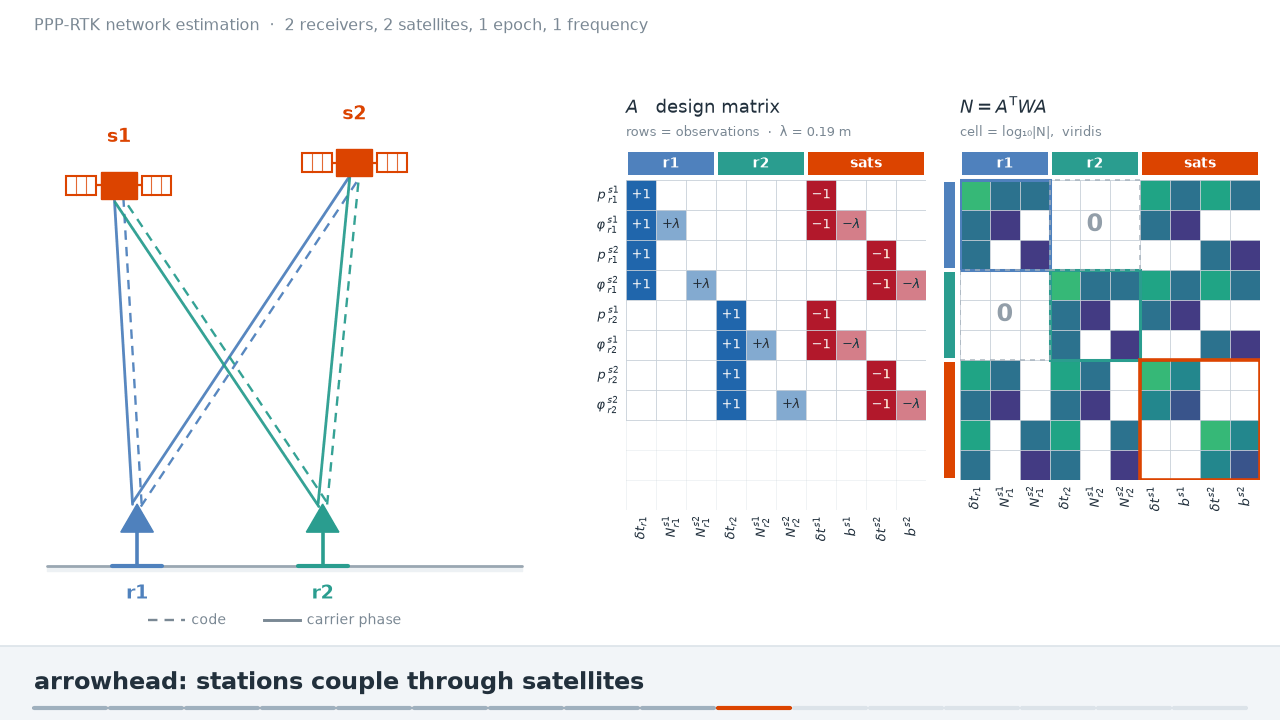
\includegraphics[width=0.49\linewidth]{toy_network_arrowhead.png}\hfill
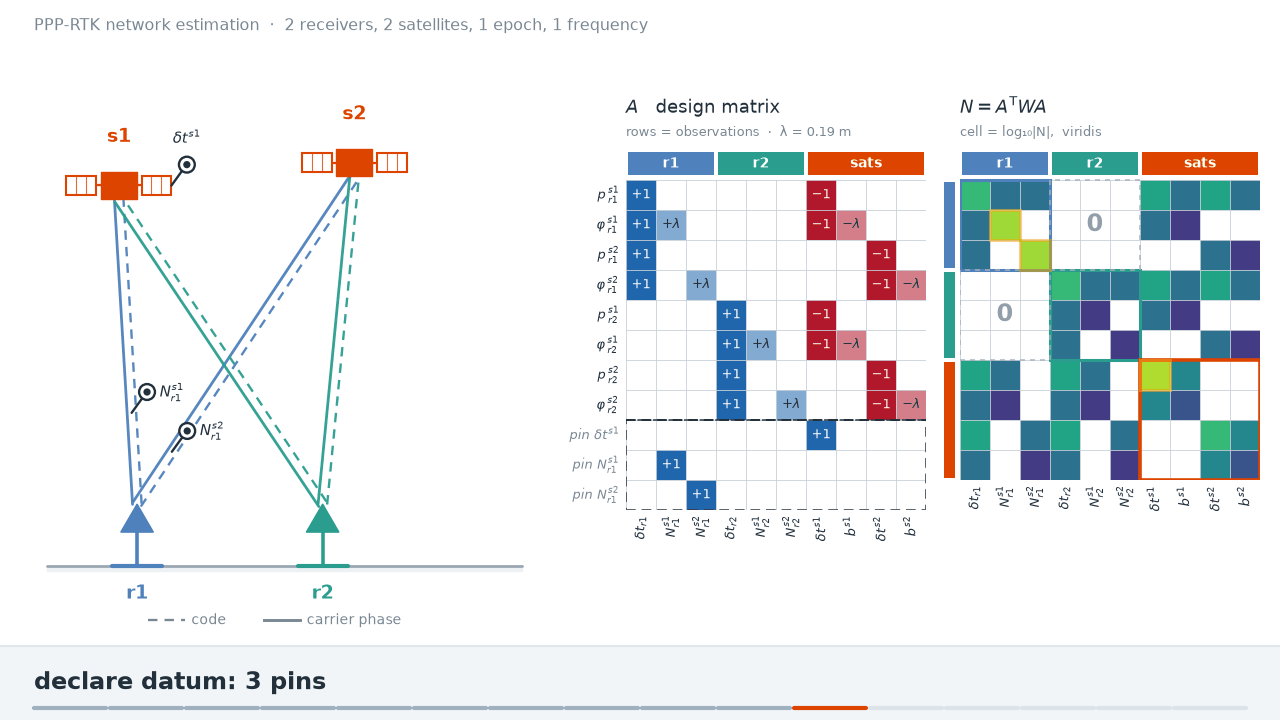
\includegraphics[width=0.49\linewidth]{toy_network_three_pins.png}
\caption{The same network with two satellites, from the project's concept
animation (\texttt{D:/GnssProcessorSupport/presentation/figures/network\_concept.gif}):
design matrix $\bm{A}$ and normal matrix $\bm{N} = \bm{A}^\Tr\bm{W}\bm{A}$. Left:
the empty blocks show that the receivers meet only through satellite terms.
Right: eight observations, ten unknowns, three null directions, removed by three
pins (the clock of satellite 1 and receiver $A$'s two ambiguities).}
\label{fig:l2-anim}
\end{figure}

\begin{question}{toy-normals}{derive}{The normal matrix and its null vector}{\ref{q:rx-clock}}
Order the unknowns $\bm{x} = [a_A, a_B, g^1, g^2, g^3, g^4]^\Tr$.
\begin{enumerate}[leftmargin=*, itemsep=1pt]
\item Write the $8\times6$ design matrix of the code rows and the normal matrix
      $\bm{N} = \bm{A}^\Tr\bm{A}$ (unit weights).
\item Show that $\bm{N}\bm{1} = \bm{0}$ for the all-ones vector. What is the rank
      of $\bm{N}$?
\item What change of the unknowns does $\bm{1}$ describe, and why can no number
      of observations of this kind fix it?
\end{enumerate}
\end{question}

\begin{question}{toy-datums}{derive}{Two reference choices, one fit}{\ref{q:toy-normals}}
\begin{enumerate}[leftmargin=*, itemsep=1pt]
\item Solve the code rows with the pin $a_A \equiv 0$, then with the pin
      $g^1 \equiv 0$.
\item Subtract the two solutions. What is the difference, in the terms of
      \cref{q:toy-normals}?
\item Compute $a_A - a_B$, $g^2 - g^1$, $g^3 - g^1$ and $a_B - g^4$ in both
      solutions. Why do they agree?
\item Under $a_A \equiv 0$, what does the estimated clock of satellite 2 equal in
      terms of the true clocks?
\end{enumerate}
\end{question}

\begin{question}{toy-phase}{derive}{Phase: the satellite phase bias needs a second receiver}{\ref{q:toy-datums}}
\begin{enumerate}[leftmargin=*, itemsep=1pt]
\item With code and phase together, count the unknowns, the observations, the
      null directions and the redundancy. Which null directions does the phase
      add?
\item With receiver $A$ alone, what does each satellite's phase determine, and
      which pair of unknowns can it not separate? What changes with receiver $B$?
\item Apply the reference choice $a_A \equiv 0$ with $N^\sat_A \equiv 0$ for every
      satellite. Compute the emitted phase bias $\bar b^\sat$ and the estimate
      $\hat N^\sat_B$ for the four satellites.
\item The physical phase bias of satellite 1 is 0.10~m and the emitted one
      10.10~m. What did it absorb? What is $\hat N^\sat_B$?
\end{enumerate}
\end{question}

\begin{question}{toy-biases}{derive}{Where the hardware biases went}{\ref{q:rx-clock}, \ref{q:rx-phase} and \ref{q:toy-phase}}
Write the network with every hardware bias explicit: receiver and satellite code
biases $B_\rx$, $B^\sat$, receiver and satellite phase biases $b_\rx$, $b^\sat$,
and the integer ambiguities. For $f$ frequencies, $n$ receivers and $m$
satellites, Odijk et al.~\cite{odijk2016estimability} count six types of null
direction (\texttt{SBASIS-THEORY-E.md}, section E2): 1a, receiver clock against
satellite clock, 1; 1b, receiver against satellite hardware biases, $2f$; 2a,
receiver clock against receiver biases, $n-1$; 3a, satellite clock against
satellite biases, $m$; 4, receiver phase bias against ambiguities, $f(n-1)$; 5,
satellite phase bias against ambiguities, $f\,m$.
\begin{enumerate}[leftmargin=*, itemsep=1pt]
\item Evaluate the six types for $f = 1$, $n = 2$, $m = 4$ and add them.
\item The worked example defined $a_\rx$, $g^\sat$ and $N^\sat_\rx$ as lumps.
      How many unknowns did the lumps remove, and how does the rank change?
      Which types are gone and which remain? Check the remainder against
      \cref{q:toy-phase}.
\end{enumerate}
\end{question}

\begin{question}{toy-user}{derive}{A user of the emitted corrections}{\ref{q:toy-datums} and \ref{q:toy-phase}}
A third receiver $C$, not in the network, has the truth $a_C = 4$ and
$N_C = (11, -4, 19, 10)$~m.
\begin{enumerate}[leftmargin=*, itemsep=1pt]
\item Compute its four code and four phase observations.
\item $C$ applies the network's satellite clocks $\hat g^\sat$ (from the choice
      $a_A \equiv 0$) and phase biases $\bar b^\sat$. Solve for its clock
      $\hat a_C$ and its ambiguities $\tilde N^\sat_C$.
\item What do $\hat a_C$ and $\tilde N^\sat_C$ equal in terms of the true values?
      Whose values does $C$'s solution carry, and does $C$ need to know it?
\end{enumerate}
\end{question}

\begin{question}{toy-setchange}{derive}{When the satellite set changes}{\ref{q:toy-datums}}
\begin{enumerate}[leftmargin=*, itemsep=1pt]
\item From the solution with $g^1 \equiv 0$, give the solution under the
      sum-to-zero choice $\sum_\sat g^\sat = 0$ over the four satellites.
\item Satellite 4 sets. Recompute both solutions with satellites 1 to 3. By how
      much does every clock move under each choice?
\item Instead satellite 1, the pinned one, sets, and the pin moves to satellite
      2. By how much does every clock move?
\item Does any of these changes move an estimable quantity? What must a user be
      told at such an epoch, and why?
\end{enumerate}
\end{question}

\lessonbox{What this lesson establishes}{%
\begin{itemize}[leftmargin=*, itemsep=0pt, topsep=2pt]
\item A reference choice is a set of pins or rows that removes the null
      directions; every admissible choice fits the data equally well.
\item Differences (estimable functions) agree under every choice; the emitted
      values carry the choice (the satellite clock carries the reference
      receiver's clock, the phase bias its ambiguity).
\item A user applying the corrections inherits the network's reference without
      knowing it: its estimates are relative to the network.
\item A sum-to-zero reference moves whenever a satellite rises or sets; a pin
      moves only when its own satellite leaves. Either move must be declared.
\end{itemize}}

% ==================================================================
\section{The real network: elimination, counting and the rank gate}\label{sec:l3}
% ==================================================================

\paragraph{Goal.} Scale the worked example up to the real network: eliminate the
stations, count the null directions, and find them again in a run.

\paragraph{The idea.} The network processor solves one joint system per epoch
over all stations (status report, step 6). The unknowns shared by all stations,
$\bm{x}_{\mathrm{B}}$, are the satellite clocks, code biases and phase biases;
each station $\rx$ has its own, $\bm{x}_\rx$: ambiguities, slant ionosphere,
zenith wet delay, receiver clock, inter-system bias and receiver code-bias
difference. Stations meet only through $\bm{x}_{\mathrm{B}}$, so the normal
matrix is an arrowhead (\cref{fig:l2-anim}, left) and each station's block is
eliminated exactly before the shared solve:
\begin{equation}
\bar{\bm{N}}_{\mathrm{BB}} = \sum_{\rx}\Big(\bm{N}^{(\rx)}_{\mathrm{BB}}
  - \bm{N}_{\mathrm{B}\rx}\bm{N}_{\rx\rx}^{-1}\bm{N}_{\mathrm{B}\rx}^\Tr\Big)
  + \bm{N}^{\mathrm{prior}}_{\mathrm{BB}},
\qquad
\bm{x}_\rx = \bm{N}_{\rx\rx}^{-1}\big(\bm{u}_\rx - \bm{N}_{\mathrm{B}\rx}^\Tr\bm{x}_{\mathrm{B}}\big).
\label{eq:l3-schur}
\end{equation}
From epoch to epoch the solution is a Kalman filter in information form. Every
epoch a check, the \emph{rank gate}, counts the eigenvalues of
$\bar{\bm{N}}_{\mathrm{BB}}$ below $\mathtt{rank\_gate\_tol}\times\lambda_{\max}$
and requires exactly the declared number (\texttt{include/network/solve/Sbasis.hpp},
\texttt{src/core/network/solve/RankGate.cpp}). A single-receiver PPP filter has
the same shape, with epochs in the place of stations (\cref{fig:l3-ppp}).

\begin{figure}[h]
\centering
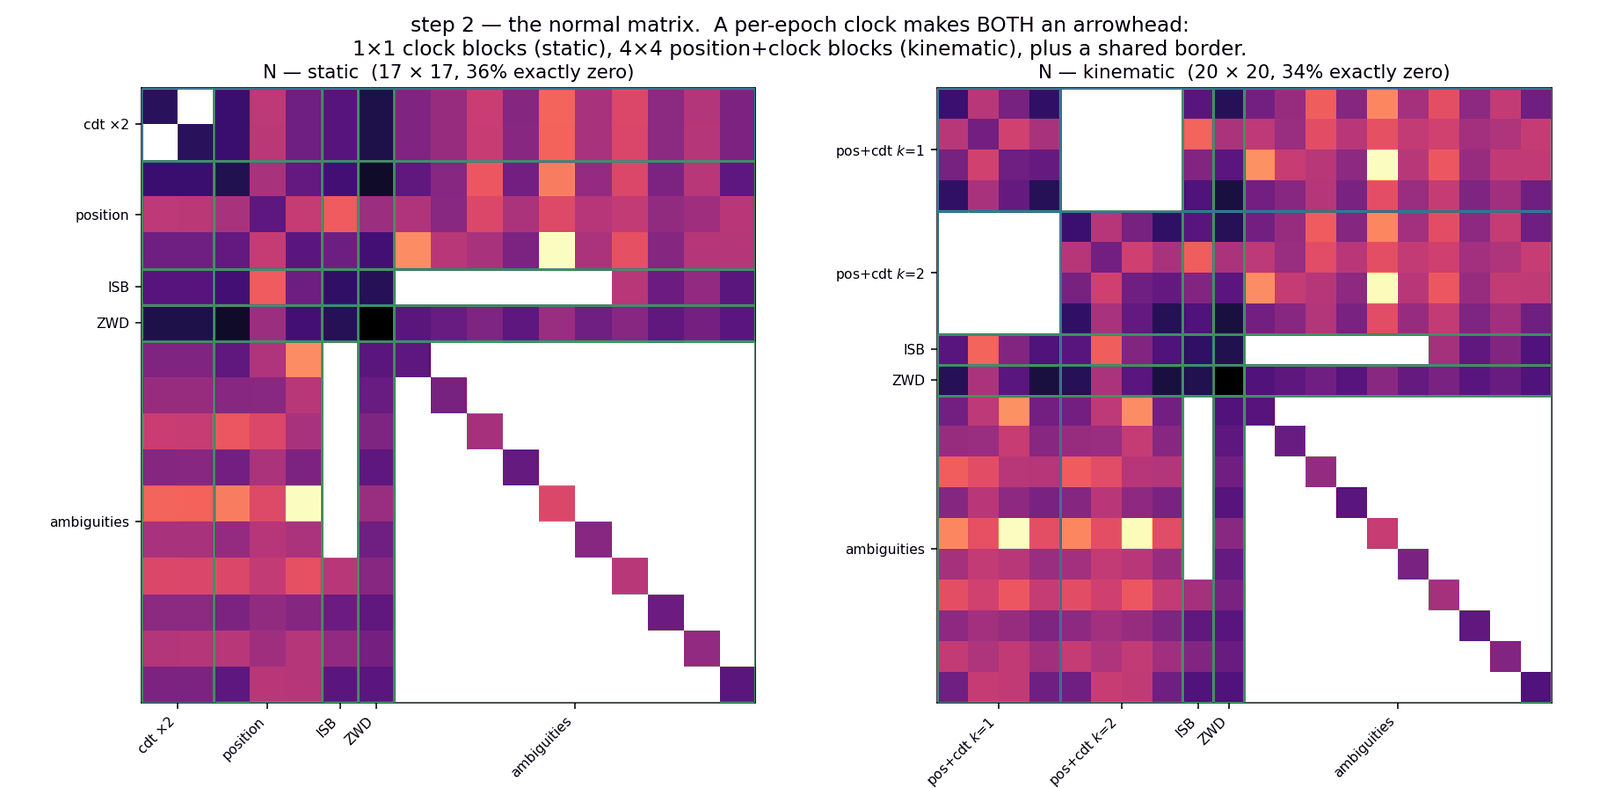
\includegraphics[width=0.62\linewidth]{per_epoch_arrowhead.png}\hfill
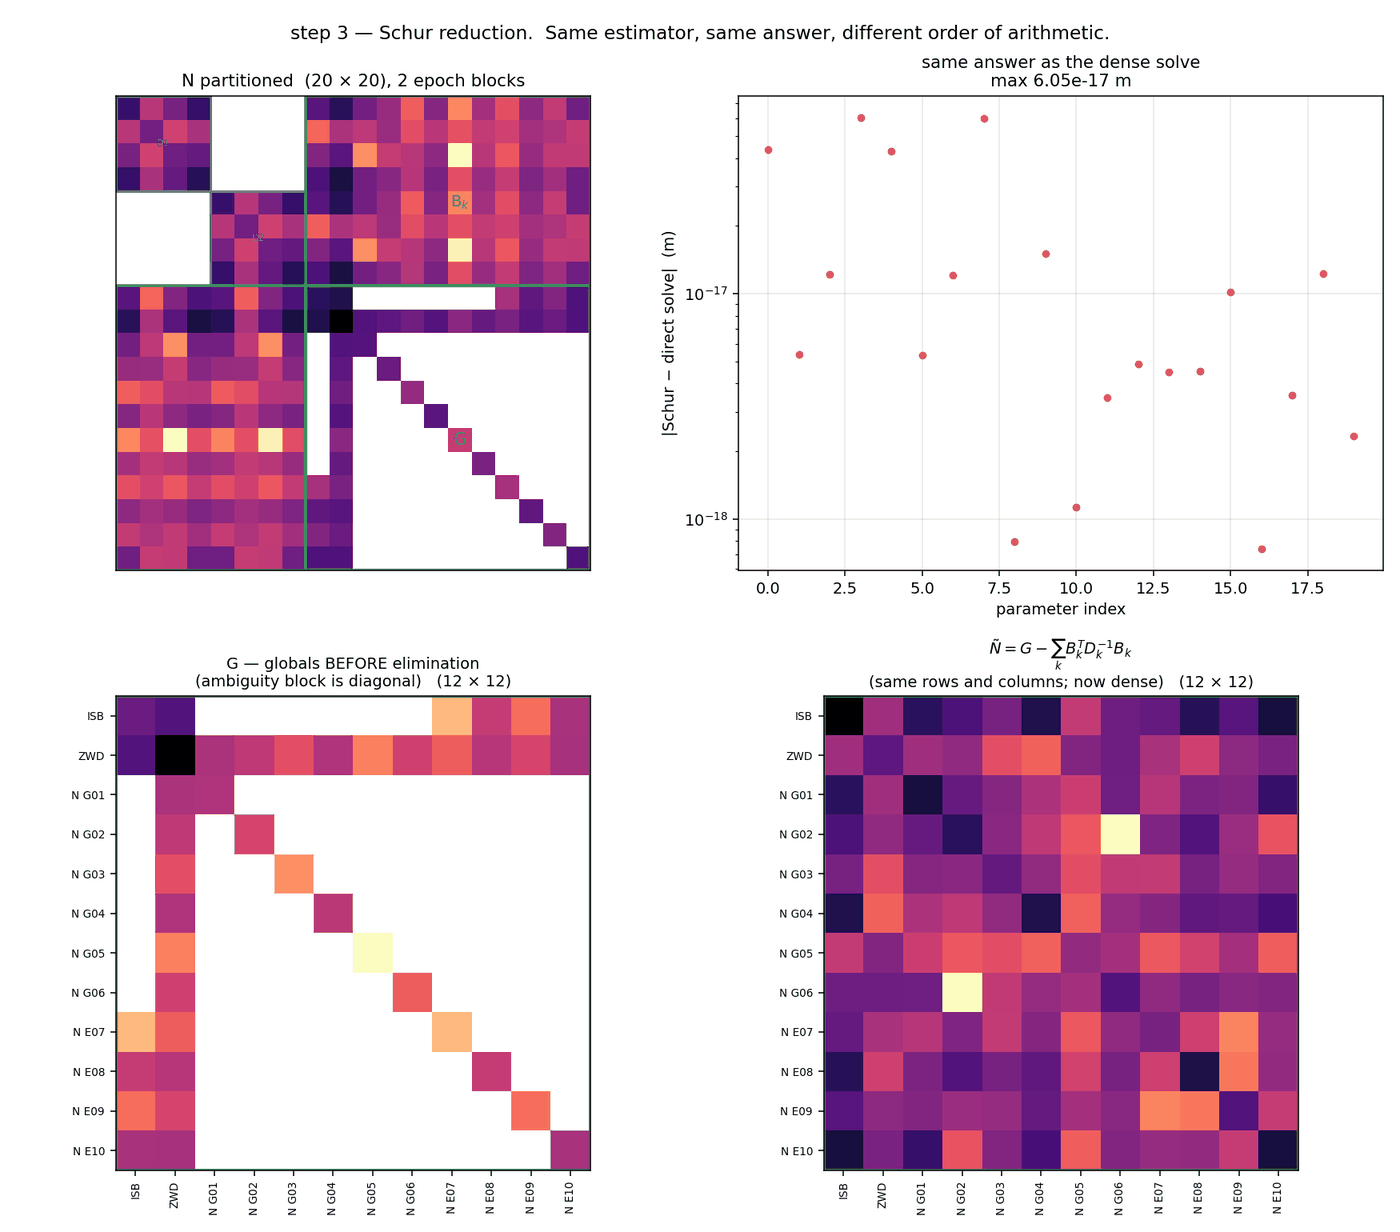
\includegraphics[width=0.36\linewidth]{schur_equals_direct.png}
\caption{Left: one receiver over two epochs; a clock per epoch makes $1\times1$
(static) or $4\times4$ (moving receiver) epoch blocks around a shared border.
Right: eliminating the blocks first gives the direct solution to $6\times10^{-17}$~m.
September 2026 illustrations.}
\label{fig:l3-ppp}
\end{figure}

\begin{question}{schur}{derive}{Eliminating the receivers}{\ref{q:toy-normals} and \ref{q:toy-datums}}
In the code system of \cref{q:toy-normals}, the receiver clocks are the local
unknowns and the satellite clocks the shared ones.
\begin{enumerate}[leftmargin=*, itemsep=1pt]
\item Compute the reduced shared normal
      $\bar{\bm{N}}_{gg} = \bm{N}_{gg} - \bm{N}_{ga}\bm{N}_{aa}^{-1}\bm{N}_{ag}$ and
      the reduced right-hand side
      $\bar{\bm{u}}_g = \bm{u}_g - \bm{N}_{ga}\bm{N}_{aa}^{-1}\bm{u}_a$ from the
      pseudorange table.
\item Find the eigenvalues of $\bar{\bm{N}}_{gg}$ and its normalized null
      eigenvector. What weight does it put on each satellite clock?
\item Solve the reduced system with $g^1 \equiv 0$, then back-substitute the
      receiver clocks with \cref{eq:l3-schur}. Compare with \cref{q:toy-datums}.
\end{enumerate}
\end{question}

\begin{question}{twosys}{derive}{Two constellations}{\ref{q:schur}}
Add Galileo satellites. Each receiver gets an inter-system bias $d^{E}_\rx$ on its
Galileo rows ($d^{G}_\rx \equiv 0$ by definition: GPS is the reference system), so
$\code^\sat_\rx = a_\rx + d^{g(\sat)}_\rx - g^\sat$.
\begin{enumerate}[leftmargin=*, itemsep=1pt]
\item Find the null directions of this system.
\item After the receiver clocks and inter-system biases are eliminated, how many
      null directions does the reduced shared normal keep, and what do they look
      like on the satellite clocks?
\item For 32 GPS and 24 Galileo satellites, what weight does each normalized
      direction put on each clock?
\end{enumerate}
\end{question}

\begin{question}{eq24}{derive}{Eq.~24 for the real network}{\ref{q:rx-iono} and \ref{q:toy-biases}}
\begin{enumerate}[leftmargin=*, itemsep=1pt]
\item Sum the six types of \cref{q:toy-biases} to obtain Eq.~24 of
      \cite{odijk2016estimability}, $1 + 2f + (1+f)(n-1+m)$. Add the
      slant-ionosphere term $n - 1 + m$ (the direction of \cref{q:rx-iono}, now at
      every receiver and every satellite).
\item \Cref{fig:l3-count} uses one constellation of 32 satellites and two
      frequencies with a slant ionosphere. Check its 369 directions for 60
      stations, 361 for 58 and 1,349 for 305.
\item The first epoch of the simulated reference run has $n = 60$, $m = 56$ (32
      GPS, 24 Galileo) and $f = 2$. What does Eq.~24 with the slant term give?
\end{enumerate}
\end{question}

\begin{figure}[h]
\centering
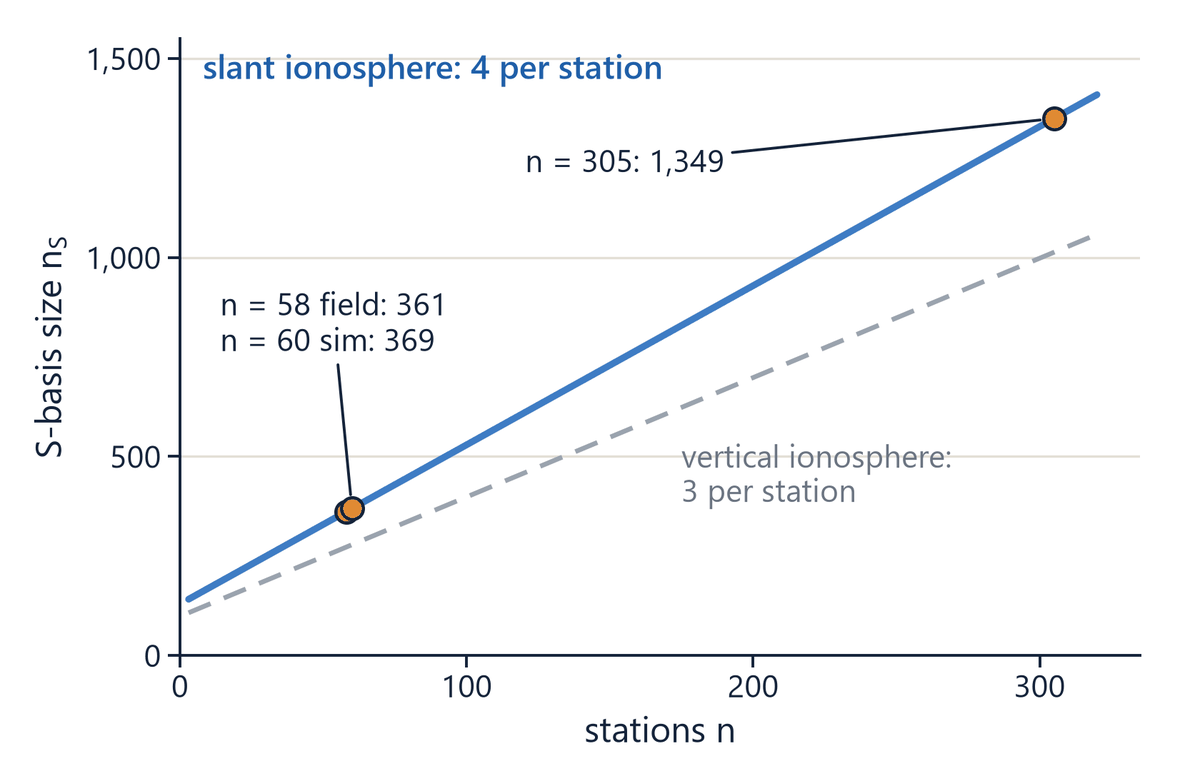
\includegraphics[width=0.48\linewidth]{undetermined_directions.png}\hfill
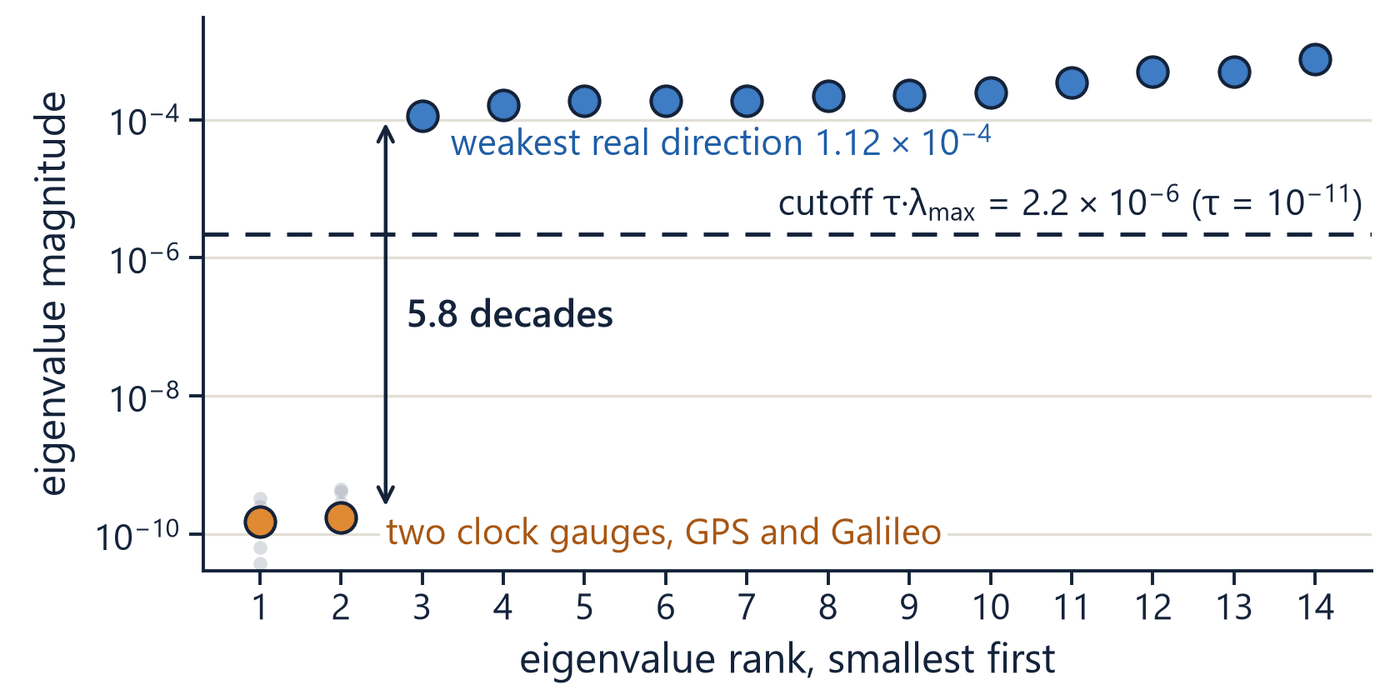
\includegraphics[width=0.5\linewidth]{rank_gate_eigenvalues.png}
\caption{Left: Eq.~24 against the number of stations, one constellation of 32
satellites, two frequencies: about four more directions per station with a slant
ionosphere, three with a vertical one (deck slide 6). Right: the rank gate on the
first real-data epoch, the 14 smallest eigenvalues of the $414\times414$ reduced
shared normal matrix: two near $10^{-10}$ (one clock direction per constellation),
the weakest real direction 5.8 decades higher, the dashed line the cutoff (deck
slide 7).}
\label{fig:l3-count}
\end{figure}

\begin{question}{inventory}{read}{The parameters as armed}{\ref{q:rx-clock} to \ref{q:rx-iono} and \ref{q:schur}}
Print the table of the simulated reference run (60 stations, GPS and Galileo,
two signals each):
\begin{cmd}
sed -n '658,686p' runs/_rf0hv15_sim6/stdout.txt
\end{cmd}
\begin{enumerate}[leftmargin=*, itemsep=1pt]
\item Map each unknown of \cref{eq:l1-code,eq:l1-phase} to a row of the table.
      Which term has no row, and where did \cref{q:rx-phase} put it?
\item How many shared and how many local columns does the run carry at its first
      epoch?
\end{enumerate}
\end{question}

\begin{question}{rankgate}{measure}{The rank gate on the real network}{\ref{q:twosys} and \ref{q:eq24}}
Run (about 9~s):
\begin{cmd}
C:/Python313/python.exe -I scripts/rf_null_space_read.py runs/_rf0hv15_sim6
grep -n "rank gate evaluated" runs/_rf0hv15_sim6/stdout.txt
\end{cmd}
\begin{enumerate}[leftmargin=*, itemsep=1pt]
\item Which two eigenvalues fall below the cutoff at the first epoch, and what
      weights do their eigenvectors carry? Compare with \cref{q:twosys}.
\item How many decades lie between the cutoff and the larger of the two, and
      between the cutoff and the weakest real direction? Does that meet the
      placement rule of \texttt{src/core/network/solve/RankGate.cpp} (lines 408
      to 410)?
\item Eq.~24 gave 465 directions; the gate declares 2. Where did the others go?
      (\Cref{q:toy-biases} holds the key; \cref{q:rows} counts the rows.)
\end{enumerate}
\end{question}

\lessonbox{What this lesson establishes}{%
\begin{itemize}[leftmargin=*, itemsep=0pt, topsep=2pt]
\item Eliminating the stations is exact; the reduced shared normal keeps the
      network's shared null directions.
\item With two constellations the shared null space is two flat clock shifts,
      weight $1/\sqrt{m_g}$ on every clock of system $g$; the real run shows
      exactly these, at 0.1767 and 0.2040.
\item Eq.~24 counts hundreds of directions; lumps, pins and priors remove almost
      all of them before the gate, which sees one per constellation. For the
      meeting: the per-epoch check confirms this count on every epoch.
\end{itemize}}

% ==================================================================
\section{The project's four reference choices}\label{sec:l4}
% ==================================================================

\paragraph{Goal.} Name the reference choices the reference configurations make,
count their rows, and find the one direction they leave to a weak prior.

\paragraph{The idea.} A reference choice is a set of constraints
$\bm{B}^\Tr\bm{x} = \bm{0}$, or pins, that picks one solution among those that fit
the data equally well. The S-transformation
$\bm{S} = \bm{I} - \bm{V}[(\bm{S}^\perp)^\Tr\bm{V}]^{-1}(\bm{S}^\perp)^\Tr$ projects
onto the estimable space along the null space $\bm{V}$; its rows are the
estimable combinations, and the reference directions carry zero variance
(\texttt{SBASIS-THEORY-E.md}, section E1, after \cite{teunissen1985generalised,
odijk2016estimability}). The record names four kinds of choice (section E3), each
with an analogue in \cref{sec:l2}: a \emph{pin} ($g^1 \equiv 0$); a
\emph{prioritized anchor} ($N^\sat_A \equiv 0$, but elected per satellite and
signal); a \emph{sum-to-zero} row ($\sum g^\sat = 0$); an \emph{ensemble}, an inner
constraint over all receivers, measured dead and deleted on 2026-10-14. The
reference configurations combine four choices:

\begin{center}\footnotesize
\begin{tabular}{@{}p{2.6cm}p{4.1cm}p{4.6cm}p{2.9cm}@{}}
\toprule
Choice & What it fixes & Settings (\texttt{golden\_sim\_refound.json}) & First epoch, simulated \\
\midrule
Clock pin & one satellite clock per constellation (the pivot); \cref{q:toy-datums,q:twosys} & no key (the default); \texttt{sticky\_pivot}, \texttt{handover\_stransform} & 2 pins (E02, G01) \\
Prioritized phase anchors, held basis & one ambiguity per satellite and signal, frozen at its basis value; \cref{q:toy-phase} & \texttt{phase\_datum\_prioritized}, \texttt{phase\_datum\_held\_basis}, \texttt{ambiguity\_vehicle} \texttt{float\_kf} & 112 pins on 18 stations \\
Code-bias datum & per satellite the ionosphere-free pin and the geometry-free pin at the broadcast $T_{GD}$; \cref{q:rx-clock,q:rx-iono} at the satellites & \texttt{estimate\_sat\_code\_bias}, \texttt{sat\_gf\_datum} \texttt{broadcast\_tgd}, \texttt{sat\_gf\_datum\_time\_linked} & $56 + 56$ rows \\
Zero-mean receiver DCB prior & the mean of the receivers' geometry-free code biases, $\sigma$ 10~m; \cref{q:rx-iono} at the receivers & \texttt{rx\_code\_bias\_datum}, \texttt{station\_prior\_before\_pd} & 120 prior entries on 60 stations \\
\bottomrule
\end{tabular}
\end{center}

One direction per station and constellation is left to the weak prior: the
station's \emph{level}, its slant ionosphere, receiver geometry-free code biases
and ambiguities shifted together. It is local, so it is eliminated before the
rank gate sees anything.

\begin{question}{theorem}{read}{The theorem in the record}{\ref{q:toy-datums}}
Read the boxed theorem of \texttt{SBASIS-THEORY-E.md}, section E1, and the
paragraph ``Datum-invariant even before choosing a datum'' of section E2.
\begin{enumerate}[leftmargin=*, itemsep=1pt]
\item What exactly is invariant, and under which choices? Where did
      \cref{q:toy-datums} show it in six unknowns?
\item Which of these are estimable before any choice: position, zenith delay,
      vertical ionosphere, a satellite clock, a satellite phase bias?
\item A differential satellite clock wander of about 47~cm was measured before
      the re-founding. Why could no change of reference cure it, and what kind of
      change can?
\end{enumerate}
\end{question}

\begin{question}{four}{read}{Four choices in the reference configuration}{\ref{q:toy-phase}, \ref{q:toy-setchange} and \ref{q:theorem}}
Confirm that the reference configurations are the generated ones, then read
\texttt{config/golden/golden\_sim\_refound.json}:
\begin{cmd}
C:/Python313/python.exe scripts/make_golden_config.py --verify
\end{cmd}
\begin{enumerate}[leftmargin=*, itemsep=1pt]
\item Through which keys does the file arm each choice of the table above?
\item How does each choice behave when a satellite rises or sets, and which of
      them, by \cref{q:toy-setchange}, would move at every rise and set?
\item Which datum-looking keys are absent from the file?
\end{enumerate}
\end{question}

\begin{question}{rows}{derive}{The rows of the first epoch}{\ref{q:rankgate} and \ref{q:four}}
The simulated case's first epoch has 56 satellites (32 GPS, 24 Galileo) at 60
stations, two signals per constellation; each satellite carries one clock, two
phase biases and two code biases.
\begin{enumerate}[leftmargin=*, itemsep=1pt]
\item How many shared columns are there, and how many rows does each choice
      contribute?
\item Account for the gate's 2: which rows act before the gate, and which after?
\item What does the solver do on an epoch whose count differs, and what would
      S-basis completion add?
\end{enumerate}
Check against lines 631, 679 to 738 and 4109 to 4112 of
\texttt{D:/GnssProcessorSupport/runs\_nom/\_rap\_scb\_g\_q6/stdout.txt}.
\end{question}

\begin{question}{cbdatum}{measure}{The code-bias datum on the corrections}{\ref{q:rx-clock} and \ref{q:rx-iono}}
Read the first epoch's code-bias records of G05 in the simulated reference case
and the G05 record of the broadcast navigation file:
\begin{cmd}
grep -n -m2 '^B,G05,' D:/GnssProcessorSupport/runs_nom/_rap_scb_g_q6/products.txt
sed -n '562,568p' data/2024-129/products/BRDC00IGS_R_20241290000_01D_MN.rnx
\end{cmd}
\begin{enumerate}[leftmargin=*, itemsep=1pt]
\item What is the ratio of the C2W record to the C1C record, what is their
      ionosphere-free combination, and how does the C1C record compare with
      $c\,T_{GD}$?
\item Where does the satellite's true geometry-free code bias go in the network
      solution, and what must a user do with its own slant ionosphere for the
      records to apply?
\end{enumerate}
\end{question}

\begin{question}{level}{derive}{The direction the shared check cannot see}{\ref{q:rx-iono}, \ref{q:schur} and \ref{q:rows}}
Card R1D (section 1) gives the loadings of the GPS level direction of station
MAJU00MHL: the receiver DCB carries a share 0.0074 of the unit direction, the
band-5 code delay $0.2392^2$ and the second-channel offset $0.1334^2$. The
receiver DCB prior has $\sigma = 10$~m.
\begin{enumerate}[leftmargin=*, itemsep=1pt]
\item What standard deviation does the prior alone give along the unit level
      direction? Check the card's ``about 116~m''.
\item A zero-mean row on the band-5 delay and the second-channel offset at the
      same $\sigma$ would add information. By what factor? Check ``about eleven
      times''.
\item Card ALD (section 3) gives $v^\Tr N v = 110$ per unit level for the coupling
      rows. What $\sigma$ follows, and which rows hold the level?
\item Why can the rank gate never see this direction, and how did it carry the
      GPS L5 event into the corrections?
\end{enumerate}
\end{question}

\lessonbox{What this lesson establishes}{%
\begin{itemize}[leftmargin=*, itemsep=0pt, topsep=2pt]
\item No admissible reference choice changes an estimable value or its variance;
      only estimation (weights, dynamics, model) can.
\item The project pins one clock per constellation, anchors one ambiguity per
      satellite and signal, pins each satellite's code biases to the broadcast
      group delay, and holds the receivers' code-bias mean with a weak prior.
\item The published code biases of the pinned pair carry no estimate; the
      ionosphere absorbs the true geometry-free bias.
\item Each station's level is held by the carried coupling, not by the datum,
      and the gate cannot see it. For the meeting: the choices are 226 rows and
      120 prior entries at the first simulated epoch, not ``a few''.
\end{itemize}}

% ==================================================================
%  Lessons 5 to 9: what a user sees, the clock, the ambiguities, and
%  the testing on simulated and real data.  Answers in answers_5_9.tex.
% ==================================================================

% ==================================================================
\section{What a user receives and sees}\label{sec:l5}
% ==================================================================

\paragraph{Goal.} Follow the corrections to a user: what it receives, what it
cannot see, and what may therefore be graded.

\paragraph{The idea.} A user positions itself with the equations of
\cref{sec:l1}, with the network's clock $C$, code bias $B$ and phase bias $P$ in
place of the satellite terms, and with its own receiver clock, slant ionosphere
and float ambiguities. The three null directions of \cref{sec:l1}, now at the
user's receiver, absorb three parts of the corrections: a change common to all
clocks of a system, a constant on a satellite's phase bias, and a geometry-free
offset of a satellite's code biases. These are the directions a reference choice
moves, so a user cannot see the choice (\cref{q:toy-user} showed it with numbers).
The S-system theory says the same of the correction covariance: its rank-one
clock and ionosphere parts ``lie in the user's own design range and are absorbed''
(\texttt{SBASIS-THEORY-E.md}, section E4). Hence standing invariant 5 of
\texttt{CLAUDE.md}: grade only datum-invariant or single-difference quantities.
The correction file declares its choices in a header line (the S line) and marks
every change of pivot with an epoch record (\texttt{E}, \texttt{datum\_changed=1}).

\begin{question}{absorb}{derive}{Three things a float user absorbs}{\ref{q:rx-clock} to \ref{q:rx-iono} and \ref{q:toy-user}}
Take the user's code and phase rows for satellite $\sat$ of system $g$, with
receiver clock, inter-system bias, slant ionosphere $I^\sat$ and float
ambiguities as unknowns, and the corrections applied.
\begin{enumerate}[leftmargin=*, itemsep=1pt]
\item Show that adding $\Delta$ to the clock $C$ of every satellite of system $g$
      changes no position.
\item Show that adding a constant $d$ to one satellite's phase bias changes no
      position, and say what changes instead.
\item Show that adding $(\delta, \mu_2\delta)$ to the two code biases of one
      satellite is absorbed, and say what that does to the user's ionosphere.
\item The status report's clock comparison (step 5) removes two means before it
      computes a standard deviation. Which two, and which of the three cases does
      each stand for?
\end{enumerate}
\end{question}

\begin{question}{sline}{read}{The header line of reference choices}{\ref{q:four}}
Line 2 of \texttt{runs/\_rf0hv15\_sim6/products.txt} is
\begin{cmd}
S,S30000SIM,1,nominal-wu93,0,0,1,0,0.05,1,COD0MGXFIN_20241290000_01D_05M_ORB.SP3+
  COD0MGXFIN_20241290000_01D_30S_CLK.CLK,E:E02,G:G01,cbjump=1,atx=igs20.atx,oref=CoM,
  discfrac=0.25,hsig=pc,cbpin=E:C1C-C5Q,cbpin=G:C1C-C2W,
  sat_gf_datum=broadcast_tgd,pbhold=2
\end{cmd}
(one line in the file). With the writer \texttt{src/core/products/NetworkProductIO.cpp}
(lines 465 to 602) and \texttt{include/products/NetworkProductEmitter.hpp}: what
does each field declare? Which fields are the reference choices of
\cref{sec:l4}? Which token does a current run add that this one lacks, and which
choice does the real-data run's S line leave undeclared?
\end{question}

\begin{question}{step}{measure}{A declared step, seen and absorbed}{\ref{q:toy-setchange} and \ref{q:absorb}}
Find the epochs at which the run declares a change of reference, then measure how
every GPS clock record moves across the GPS one (tow 276150):
\begin{cmd}
awk -F, '/^E,/ && $7=="1" {print NR": "$0}' runs/_rf0hv15_sim6/products.txt
C:/Python313/python.exe - <<'EOF'
import statistics as st
d, t = {}, None
for line in open('runs/_rf0hv15_sim6/products.txt'):
    f = line.rstrip('\n').split(',')
    if f[0] == 'E':
        t = round(float(f[2]) / 30) * 30
    elif f[0] == 'C' and f[1].startswith('G') and t in (276120, 276150):
        d.setdefault(f[1], {})[t] = float(f[2])
s = [v[276150] - v[276120] for v in d.values() if len(v) == 2]
print(len(s), 'satellites, mean step %.4f m, sd after the mean %.4f m'
      % (st.mean(s), st.pstdev(s)))
EOF
\end{cmd}
\begin{enumerate}[leftmargin=*, itemsep=1pt]
\item How large is the step of the GPS clock records, and how much of it is left
      after the per-system mean is removed?
\item Which move of \cref{q:toy-setchange} is this, and what absorbs it at a
      user?
\item Why would a grade of raw clock steps call this epoch a 1.6~m defect?
\end{enumerate}
\end{question}

\begin{question}{refsat}{measure}{The reference satellite in every chord}{\ref{q:toy-datums} and \ref{q:absorb}}
The network's double-difference trace (\texttt{network\_dd\_fractional.csv})
differences every satellite against one reference satellite.
\begin{enumerate}[leftmargin=*, itemsep=1pt]
\item Derive: if every satellite's error has variance $\sigma^2$ and the reference
      satellite's $\sigma_{\mathrm{ref}}^2$, what is the variance of one chord and
      the correlation between two chords?
\item Run (about 12~s) and compare the L1C error as traced and reference-free
      (median $|e|$ in cycles, and the share that rounds to the right integer),
      over all epochs and over the last quarter:
\begin{cmd}
C:/Python313/python.exe scripts/simnet_amb_integer.py runs/simnet60_quiet_col_24h \
    --run runs/_rf0hv15_sim6 --ref-free
\end{cmd}
\item Why does a grade on the traced chords report the reference satellite's
      error?
\end{enumerate}
\end{question}

\lessonbox{What this lesson establishes}{%
\begin{itemize}[leftmargin=*, itemsep=0pt, topsep=2pt]
\item A float user absorbs a system-common clock change, a constant on a phase
      bias and a geometry-free code-bias offset; the reference choice is
      invisible to it.
\item A declared step of 1.63~m on every GPS clock leaves 3~mm after the
      per-system mean: grade datum-invariant quantities, never raw steps.
\item A double difference built on one reference satellite carries that
      satellite's error in every chord: grade reference-free. For the meeting:
      every number in the report is graded this way.
\end{itemize}}

% ==================================================================
\section{The satellite clock in time}\label{sec:l6}
% ==================================================================

\paragraph{Goal.} See how the network ties each satellite clock to its past, what
the phase-clock hold passes to a user, and why the clock's precision today is the
a priori clock product's.

\paragraph{The idea.} Three mechanisms shape the per-satellite part of the
clock, the part a user cannot absorb.
\begin{enumerate}[leftmargin=*, itemsep=1pt]
\item \emph{The temporal anchor} (card Q3, \texttt{network.clock\_temporal\_anchor}).
      Without it the clock is re-estimated from each epoch's data: the step
      between epochs was 9.23~cm per 30~s, because the clock's own process noise
      (\texttt{sat\_clock\_q}, $10^{-3}$~m$^2$/s) never binds. The anchor folds the
      previous epoch's clock in as a prior with variance
      $\max(\mathrm{var} + q\,\Delta t,\ \mathrm{floor})$ and
      \texttt{clock\_anchor\_q} $= 2.9\times10^{-8}$~m$^2$/s, a value measured from
      the clock's structure function (\cref{fig:l6-clock}, left).
\item \emph{The exact coupling update} (card CTU,
      \texttt{carry\_coupling\_exact\_update}). Carried station rows used to age the
      clock at $10^{-3}$~m$^2$/s while the shared solve folded it at
      $2.9\times10^{-8}$; the level froze. The exact update lets it converge at the
      anchor's rate (\cref{fig:l6-clock}, right).
\item \emph{The phase-clock hold} (cards PBH and LAH,
      \texttt{emit\_pb\_hold\_phase\_clock}). Between declared resets the network
      keeps each satellite's clock minus phase bias, $C - P$, constant up to a
      common mode, so a user's phase rows follow the a priori clock.
\end{enumerate}
Card SCB (24~October) made the consequence measurable on a simulated data set with
injected satellite clock error (offset $\sigma$ 0.5~m, rate $\sigma$
$10^{-5}$~m/s, random walk $3\times10^{-8}$~m$^2$/s).

\begin{figure}[h]
\centering
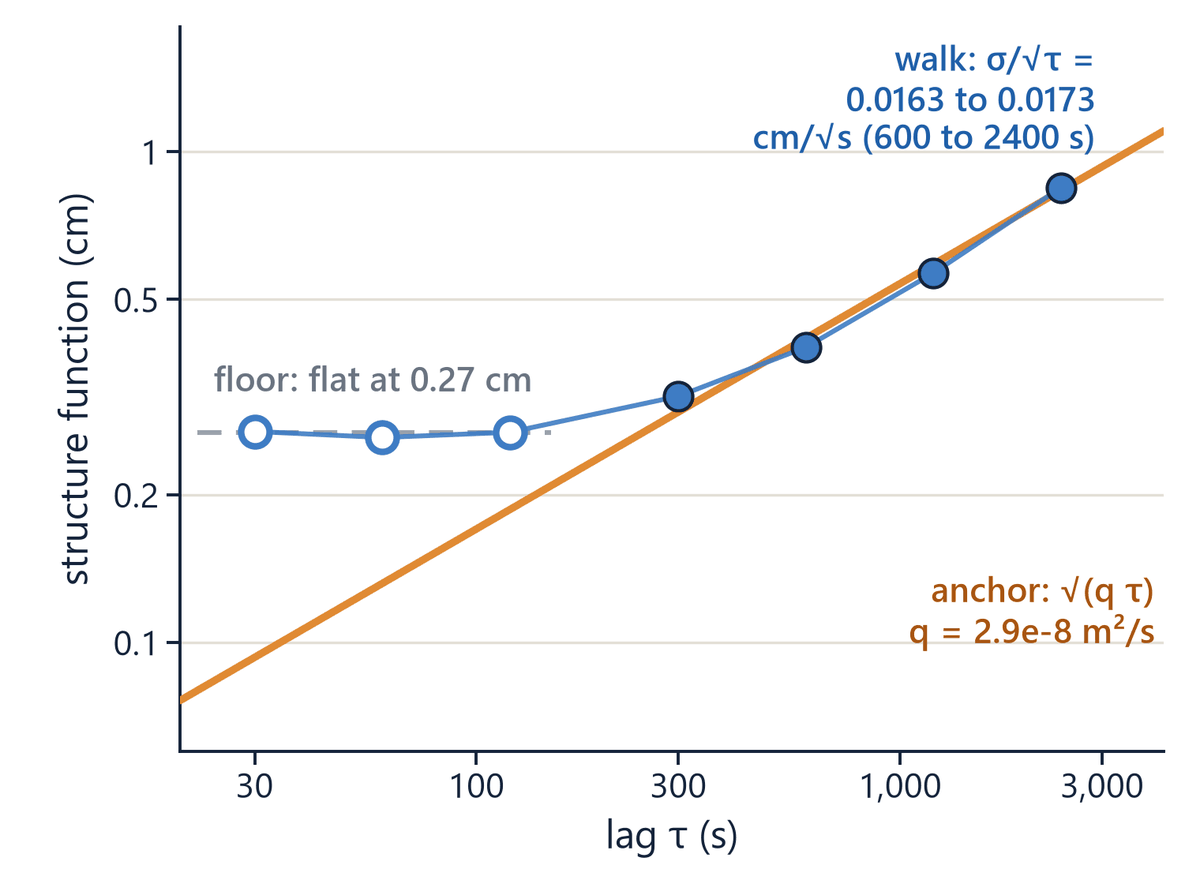
\includegraphics[width=0.44\linewidth]{clock_structure_function.png}\hfill
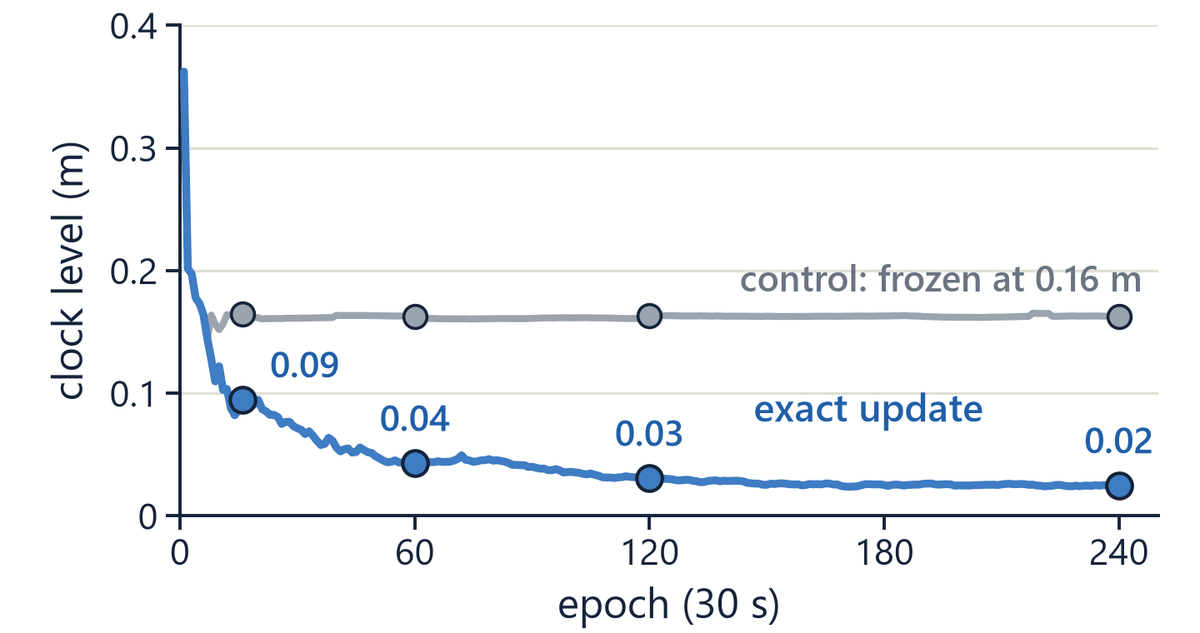
\includegraphics[width=0.54\linewidth]{sim_clock_level_update.png}
\caption{Left: structure function of the network's satellite clock correction
against lag: a floor of 0.27~cm from 30 to 120~s, then growth along the anchor's
line $\sqrt{q\tau}$, $q = 2.9\times10^{-8}$~m$^2$/s (deck slide 11). Right:
simulated network, error of the clock level by epoch, graded from 00:30:15: the
control freezes at 0.16~m, the exact coupling update falls to 0.02~m by epoch 240
(deck slide 10).}
\label{fig:l6-clock}
\end{figure}

\begin{question}{qstep}{derive}{A spectral density as a step}{}
\texttt{clock\_anchor\_q} is $2.9\times10^{-8}$~m$^2$/s and the epoch 30~s.
\begin{enumerate}[leftmargin=*, itemsep=1pt]
\item What is the $1\sigma$ random-walk step per epoch, and the $1\sigma$
      accumulation over 6~h?
\item The injected rate on the clock data set has $\sigma$ $10^{-5}$~m/s, 0.30~mm
      per epoch, which card SCB calls ``inside the golden anchor's permitted
      0.93~mm per epoch''. After how many epochs does a $10^{-5}$~m/s drift exceed
      the walk's $1\sigma$ accumulation? Why does comparing step sizes not
      guarantee that the anchor follows the drift?
\end{enumerate}
\end{question}

\begin{question}{tau}{derive}{A spectral density as a time constant}{\ref{q:qstep}}
Treat the anchored clock as a scalar random walk observed once per epoch with
noise variance $R = (9.23~\mathrm{cm})^2/2$ (the pre-anchor step is the difference
of two independent epoch estimates). Use the steady-state gain
$K = \sqrt{q\,\Delta t/R}$ of \texttt{docs/cards/raim-qc/DAY129-FRAME-ANATOMY.md}
(lines 138 to 143).
\begin{enumerate}[leftmargin=*, itemsep=1pt]
\item What are $K$ and the time constant $\Delta t/K$?
\item What error does a $10^{-5}$~m/s drift leave? Compare with the coefficient
      card SCB measured for the reference configuration, 2127~s.
\item What does the same argument give for the self-contained regime's
      $q = 5\times10^{-6}$~m$^2$/s? Card SCB measured 52~s.
\end{enumerate}
\end{question}

\begin{question}{hold}{derive}{What the phase-clock hold passes to the user}{\ref{q:absorb} and \ref{q:qstep}}
\texttt{include/network/emit/PbHold.hpp} (lines 60 to 66) writes the held phase
bias of a satellite as $P(t) = p(t_0) + [\tilde c(t) - \tilde c(t_0)]$, with
$\tilde c = c - M$ the estimated clock minus its system mean.
\begin{enumerate}[leftmargin=*, itemsep=1pt]
\item Show what $C - P$ is between resets, and what a user's phase rows see when
      the a priori clock is $a(t)$ and the truth $a(t) + e(t)$.
\item On the clock data set $e(t)$ is a rate ($\sigma$ $10^{-5}$~m/s) plus a random
      walk ($3\times10^{-8}$~m$^2$/s). What rms error does the hold pass to the
      phase rows in hour 6 (5 to 6~h after the reset)? Card SCB, section 8,
      measured 0.201~m for GPS.
\item Lines 311 to 319 of \texttt{src/core/config/GnssConfigLoadNetwork.cpp}
      enforce a precondition on the hold. Which, and why does part 1 make it
      necessary? Which token of the S line declares the hold in force?
\end{enumerate}
\end{question}

\begin{question}{postures}{measure}{Two postures on the clock data set}{\ref{q:tau} and \ref{q:hold}}
Run the clock grader on the reference case and on the self-contained regime, both
on the clock data set (a few seconds each):
\begin{cmd}
C:/Python313/python.exe -B scripts/simnet_clock_truth_grade.py \
    --fixture D:/GnssProcessorSupport/fixtures/simnet60_clk_col_24h \
    --run D:/GnssProcessorSupport/runs_nom/_rap_scb_g_k6
C:/Python313/python.exe -B scripts/simnet_clock_truth_grade.py \
    --fixture D:/GnssProcessorSupport/fixtures/simnet60_clk_col_24h \
    --run D:/GnssProcessorSupport/runs_nom/_rap_scb_c_k6
\end{cmd}
Read for each the clock level at hour 6, the rms of the per-satellite mean
errors, the correlation of the mean error with the drawn rate, and the user's
hourly error in hours 3 to 6. Which posture follows the drift? Why is the
reference case's user error so much larger than its clock error? What do these
lines not show?
\end{question}

\begin{question}{nbp}{derive}{The cost of leaving the final clock, on real data}{\ref{q:postures}}
Card NBP, section 12 (lines 212 to 219), splits the cost of the native
broadcast-clock posture over days 130 to 132 into three steps: the self-contained
regime $+0.0024$~m, removing satellite G01 $-0.0007$~m, the broadcast clock in place
of CODE's $+0.0099$~m. The pooled median of the whole change is $+0.0171$~m (line
176).
\begin{enumerate}[leftmargin=*, itemsep=1pt]
\item Why do the steps not add to the total? Which part is the clock's
      information?
\item Against which reference configuration, which days and which hours was the
      1.7~cm measured, and what does the first hour add?
\end{enumerate}
\end{question}

\lessonbox{What this lesson establishes}{%
\begin{itemize}[leftmargin=*, itemsep=0pt, topsep=2pt]
\item $q = 2.9\times10^{-8}$~m$^2$/s is a 0.93~mm step per epoch and, against the
      epoch noise, a time constant of about 35~min.
\item The phase-clock hold hands a user the a priori clock's motion: a wrong a
      priori clock reaches the phase rows one to one, so the hold is valid only
      with a precise a priori clock.
\item The self-contained postures estimate the clock to about 2~cm on simulated
      error but are not armed; on real data, replacing CODE's clock costs 1.7~cm
      at the median. For the meeting: the clock's precision is CODE's.
\end{itemize}}

% ==================================================================
\section{Float ambiguities and integers}\label{sec:l7}
% ==================================================================

\paragraph{Goal.} See why the network keeps its ambiguities float, what a complete
set of integers would buy, and why the corrections carry no integers yet.

\paragraph{The idea.} In the uncombined model every phase row carries both the
slant ionosphere and an ambiguity, and on GPS L1 and L2 the two enter in nearly
the same direction: a common L1 and L2 cycle moves the phase by $(\lambda_1,
\lambda_2) = (0.1903, 0.2442)$~m, the ionosphere along $(1, \mu_2)$ with $\mu_2 =
1.6469$. With a free slant ionosphere per line of sight, the integers become
visible only once the double-differenced ionosphere is known to about 0.1 L1
cycle. The re-founding chose the \emph{float vehicle} (card RF-1): each ambiguity
is a float state of its station block with a joint covariance, a floored birth
prior and zero process noise; integers are graded, not fixed. \Cref{q:toy-user}
showed where a user's integer property comes from: the network's pins.

\begin{figure}[h]
\centering
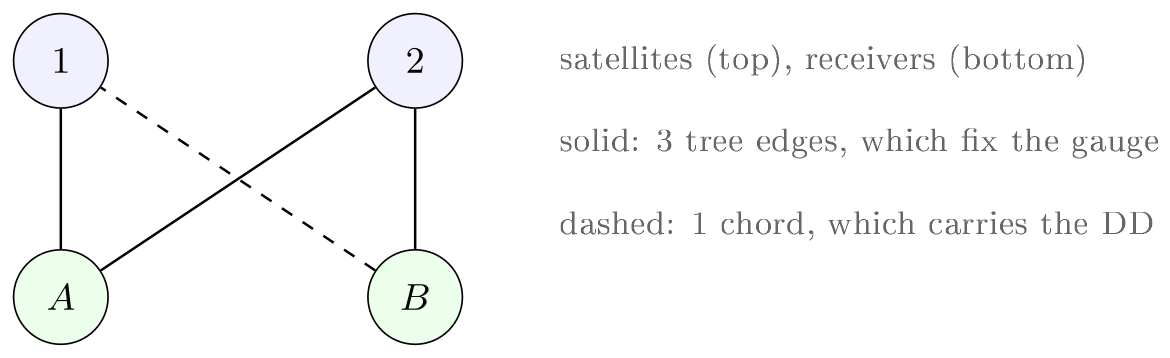
\includegraphics[width=0.46\linewidth]{observation_graph_cycle.png}\hfill
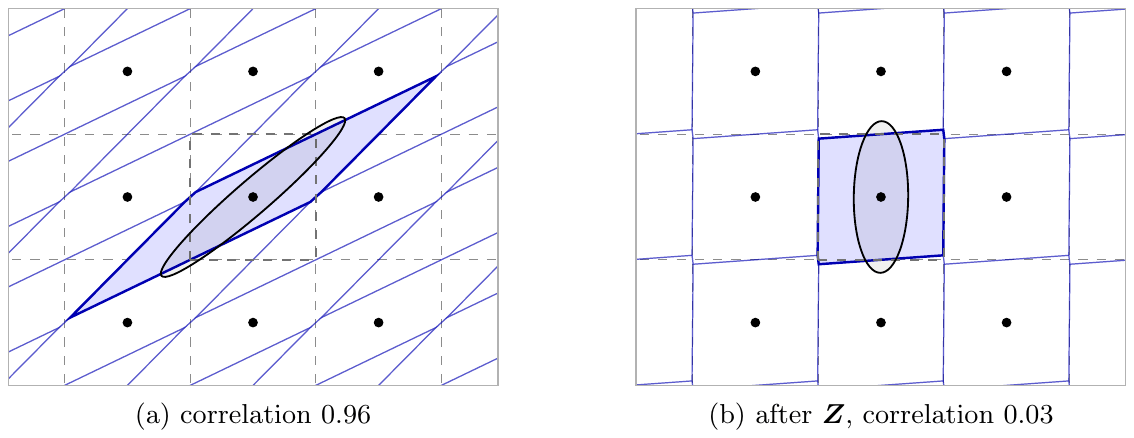
\includegraphics[width=0.5\linewidth]{pull_in_regions.png}
\caption{Left: the smallest observation graph with a cycle: satellites 1 and 2
(top), receivers $A$ and $B$ (bottom); the three solid arcs form a spanning tree
whose ambiguities the reference choice fixes, the dashed chord carries the one
double difference the data determine (\texttt{docs/report/network\_carry.tex},
figure 1). Right: a two-dimensional integer search; at correlation 0.96 the error
ellipse is long and the search's pull-in region a long parallelogram, unlike the
rounding squares (dashed); after the decorrelating transformation $\bm{Z}$ the
two nearly agree (\texttt{docs/report/linear\_algebra.tex}, figure 3; a generic
example).}
\label{fig:l7}
\end{figure}

\begin{question}{nl}{derive}{Why an integer is mostly ionosphere}{\ref{q:rx-phase} and \ref{q:rx-iono}}
From $f_1 = 1575.42$~MHz and $f_2 = 1227.60$~MHz, compute $\lambda_1$, $\lambda_2$
and $\mu_2$, the angle between the ionosphere direction $(1, \mu_2)$ and the
common-cycle direction $(\lambda_1, \lambda_2)$ in metres of phase, its cosine,
and the part of one common L1 and L2 cycle that is orthogonal to the ionosphere.
Card ARL (line 43) calls a narrow-lane integer ``99.3\,\% ionosphere''. Is that a
share of amplitude or of variance?
\end{question}

\begin{question}{cycles}{derive}{An ionosphere error in cycles}{\ref{q:nl}}
A double-difference L1 ionosphere error $d$ (metres) is absorbed by the
ambiguities.
\begin{enumerate}[leftmargin=*, itemsep=1pt]
\item What are the L1 and wide-lane ($L1 - L2$) errors in cycles for
      $d = 0.4233$~m (no pin) and $d = 0.0419$~m (every ambiguity pinned)? Check
      the factors against \texttt{docs/cards/raim-qc/T3-IONO-MECHANISM.md} (lines
      326 to 331).
\item Instantaneous resolution needs about 0.1 L1 cycle. What is that in metres
      and in TECU, and by what factor does the no-pin case miss it?
\end{enumerate}
\end{question}

\begin{question}{pins}{derive}{Integer pins and float pins}{\ref{q:toy-user} and \ref{q:four}}
Work \cref{q:toy-user} in cycles, with a receiver phase bias $\beta_\rx$ (the same
for every satellite), so that $N^\sat_\rx = z^\sat_\rx + \beta_\rx$ with
$z^\sat_\rx$ an integer. Let the network pin $N^\sat_A \equiv \zeta^\sat$ instead of 0.
\begin{enumerate}[leftmargin=*, itemsep=1pt]
\item What does the network emit as $\bar b^\sat$, and what does the user $C$
      estimate as $\tilde N^\sat_C$?
\item Form the difference between satellites $\sat$ and $k$ at $C$. When is it an
      integer?
\item The reference configuration pins each anchor ambiguity at its own float
      value (\texttt{docs/network\_ambiguity\_resolution\_design.md}, line 335).
      What does part 2 predict for its corrections? What does card IRD (sections
      1 to 3) propose instead?
\end{enumerate}
\end{question}

\begin{question}{oracle}{read}{Complete and partial pins}{\ref{q:cycles}}
Read sections 0 and 8.1 of \texttt{docs/SPEC\_oracle\_pin.md}. What is the
``integer-information deficit'', which row of its table carries it, and why is the
raw per-line-of-sight error (2.73~m) the wrong row? What do the partial pins
(L5Q alone; L1C with L2W; one station; one satellite) show, and on which simulated
data set were the numbers produced?
\end{question}

\begin{question}{null}{measure}{Integers in the float, none in the corrections}{\ref{q:pins}}
Run (each under 10~s):
\begin{cmd}
C:/Python313/python.exe scripts/simnet_wire_integer_consistency.py \
    runs/simnet60_quiet_col_24h --run runs/_rf0hv15_sim6 --bands L1C,L2W \
    --systems G --wl --nl --null-mc 500 --start-hms 00:30:15
C:/Python313/python.exe scripts/simnet_producer_ar_grade.py runs/simarl_r2 \
    --run runs/_rap_arl_r2dp --settle-h 1
\end{cmd}
The first grades the published GPS phase biases for integer consistency (the
fraction of wide-lane and narrow-lane combinations against a uniform null; a set
of perfect corrections reads 0.000). The second grades the log-only integer search
of card ARL. What does each print, and what do the two together say about where
the integers are?
\end{question}

\lessonbox{What this lesson establishes}{%
\begin{itemize}[leftmargin=*, itemsep=0pt, topsep=2pt]
\item An L1 and L2 integer step lies $6.66^\circ$ from the ionosphere direction;
      with a free slant ionosphere the integers need a double-differenced
      ionosphere to 0.117~TECU.
\item A user's between-satellite ambiguity is an integer only if the network's
      pins are integers; the reference configuration pins float values, so its
      corrections sit at the uniform null.
\item The network's float solution holds integers (a log-only search fixes 42\,\%
      on a simplified simulation, none wrongly). For the meeting: no integers are
      published or fixed on real data.
\end{itemize}}

% ==================================================================
\section{Testing on simulated data}\label{sec:l8}
% ==================================================================

\paragraph{Goal.} See what the simulated network certifies, where a simulated run
starts and is graded, and how much error the network adds above the user's own
floor.

\paragraph{The idea.} The simulated data set \texttt{runs/simnet60\_quiet\_col\_24h}
holds 60 network stations and the test station SZZ000SIM at 30~s from 00:00:30
(\cref{fig:l8}, left). It is \emph{quiet}: no cycle slips and no satellite clock
error, because its truth clock is the CODE product that the network also takes as
its a priori clock. The simulator extrapolated the satellite positions outside its
SP3 window for its first epochs; the reference case is graded from 00:30:15. The
network reports clocks and biases in its own reference choices, so truth is moved
into that basis before any comparison. The simulator also writes a set of perfect
corrections, so the same test station can be positioned with both sets
(\cref{fig:l8}, right).

\begin{figure}[h]
\centering
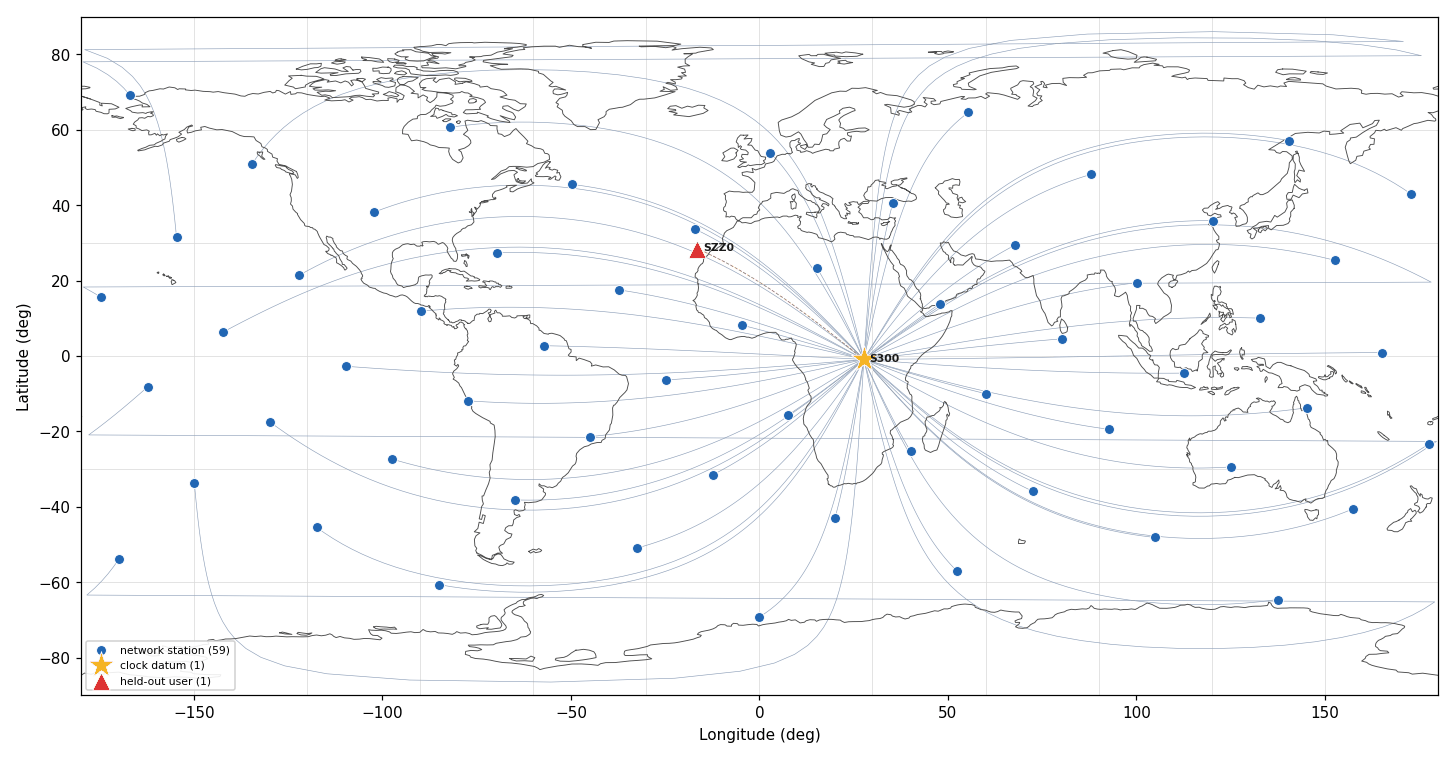
\includegraphics[width=0.42\linewidth]{sim_network_map.png}\hfill
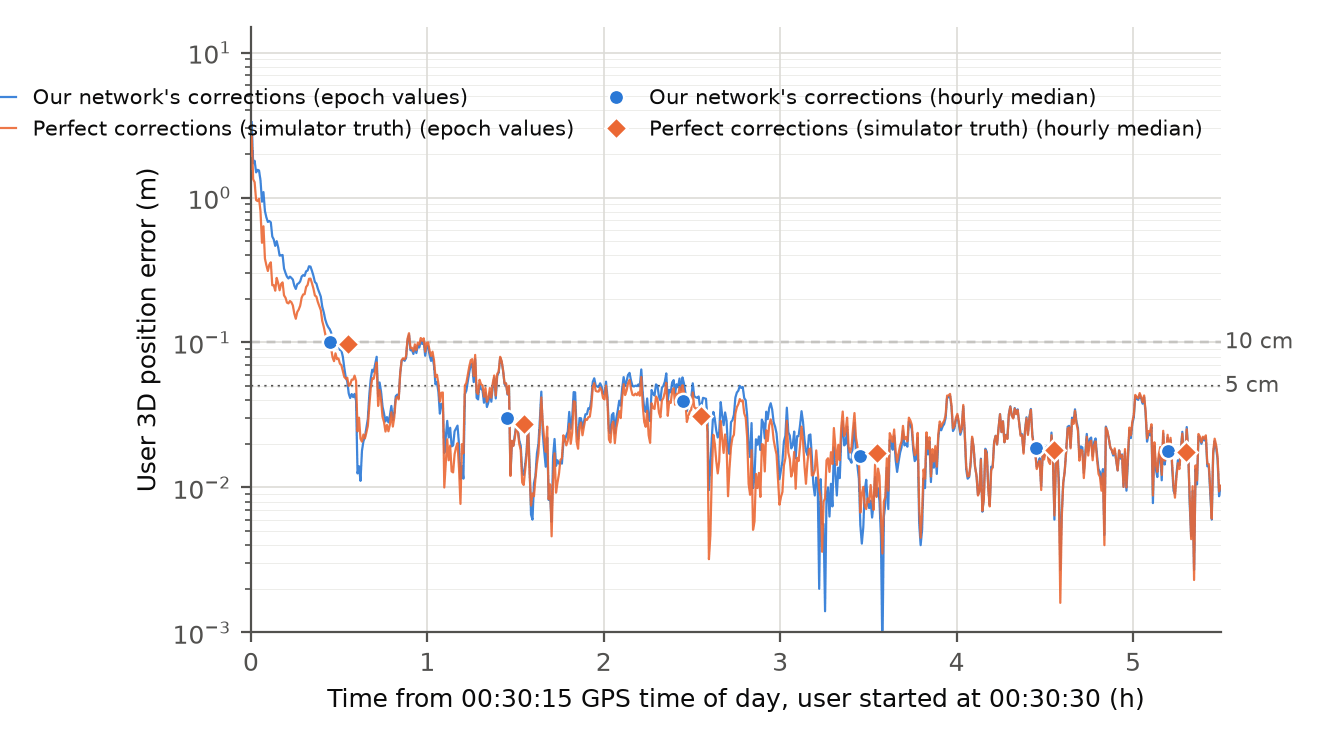
\includegraphics[width=0.56\linewidth]{sim_user_restarted.png}
\caption{Left: the simulated network, 59 stations and the clock-datum station
S30000SIM (star); the test station SZZ000SIM (triangle) is left out (deck slide
15). Right: SZZ000SIM with our network's corrections (blue) and with perfect
corrections (orange), user started at 00:30:30; lines are epochs, markers hourly
medians (\texttt{results/t2/plain/t2\_sim\_floor\_restart.png}).}
\label{fig:l8}
\end{figure}

\begin{question}{quiet}{read}{What the quiet simulation cannot test}{\ref{q:hold}}
Read card SCB, section 1 and the start of section 2 (lines 17 to 25), and
\texttt{results/t2/results.md} (lines 123 to 126). What makes the clock untestable
on the quiet data set, and what does its 0.9~cm agreement certify instead? Check
the absence of injected clock error directly:
\begin{cmd}
ls runs/simnet60_quiet_col_24h/*/truth_satclock.csv 2>/dev/null | wc -l
ls D:/GnssProcessorSupport/fixtures/simnet60_clk_col_24h/*/truth_satclock.csv | wc -l
\end{cmd}
\end{question}

\begin{question}{start}{derive}{Where a simulated run starts}{}
\begin{enumerate}[leftmargin=*, itemsep=1pt]
\item The data set's first epoch is tow 259230 (00:00:30). An epoch is reached when
      its elapsed time since the first epoch is at least the offset
      (\texttt{include/math/TimeUtils.hpp}, lines 416 to 448). At which tow and
      time do \texttt{network.start\_offset\_hours} 0.504167 and 0.4958333333 start
      a run? What does the ``half-epoch back-off'' do?
\item Count the extrapolated epochs. The geometry log warns only when the
      extrapolation exceeds half the SP3 interval
      (\texttt{src/core/model/ModelGeometry.cpp}, line 1204):
\begin{cmd}
grep "Position extrapolation" \
    runs/simnet60_quiet_col_24h/SZZ000SIM/logs/geometry.log \
  | sed -E 's/.*tow ([0-9.]+):.*/\1/' \
  | awk '{c[int(($1+15)/30)*30]++} END{for(e in c) print e,c[e]}' | sort -n
\end{cmd}
      How many epochs are logged, how many precede the SP3 window (which opens at
      tow 259500), and is ``faulty in the first 30 minutes'' the right description?
\end{enumerate}
\end{question}

\begin{question}{basis}{measure}{The published baseline's clock in the network's basis}{\ref{q:cbdatum}, \ref{q:absorb} and \ref{q:start}}
Run the clock grader on the published simulated baseline (started 00:00:30) and on
card SCB's quiet case (started 00:31:00):
\begin{cmd}
C:/Python313/python.exe -B scripts/simnet_clock_truth_grade.py \
    --fixture runs/simnet60_quiet_col_24h --run runs/_rf0hv15_sim6 --hours 6
C:/Python313/python.exe -B scripts/simnet_clock_truth_grade.py \
    --fixture runs/simnet60_quiet_col_24h \
    --run D:/GnssProcessorSupport/runs_nom/_rap_scb_g_q6
\end{cmd}
Compare the clock level by hour and the rms of the per-satellite mean errors.
Rerun the first with \texttt{--no-ds}: what does the datum share remove, and why
is it added to the truth rather than subtracted from the estimate? Why does the
first run's user not show its per-satellite constants?
\end{question}

\begin{question}{floor}{derive}{The network's cost and the user's floor}{\ref{q:start}}
From \texttt{results/t2/results.md} (lines 195 to 206), the hourly 3D medians with
the user restarted at 00:30:30, in metres: perfect corrections 0.0983, 0.0275,
0.0311, 0.0173, 0.0181, 0.0176; our network 0.1013, 0.0301, 0.0396, 0.0166, 0.0186,
0.0178. Compute the network's cost per hour, the largest cost and the floor in
hours 4 to 6. In which component does the floor sit (\texttt{results/t2/metrics.csv})?
\end{question}

\lessonbox{What this lesson establishes}{%
\begin{itemize}[leftmargin=*, itemsep=0pt, topsep=2pt]
\item The quiet simulation has no clock error to estimate; it certifies the
      algebra and the biases.
\item Nine epochs are extrapolated; 00:30:15 is a grading origin, and a run
      started at 00:00:30 keeps per-satellite clock constants of 0.32~m that no
      float user can see.
\item With perfect corrections as the control, the network adds at most 0.9~cm;
      the 1.7 to 1.8~cm floor is the user side's, in the height. For the
      meeting: one realization, no slips, no clock error.
\end{itemize}}

% ==================================================================
\section{Real data, and what may be claimed}\label{sec:l9}
% ==================================================================

\paragraph{Goal.} Grade the real-data result the way the project does, and put the
course together into what the presentation may claim.

\paragraph{The idea.} The real-data reference case
(\texttt{config/golden/golden\_field\_refound.json}, run \texttt{runs/\_rf0hv15\_field6})
processes 58 IGS stations on 8 May 2024, GPS L1/L2 and Galileo E1/E5a. The test
station WTZZ00DEU is left out of the network and positioned as a moving receiver
from the clock and bias records, without integer fixing and with its own float
ionosphere; it shares its site with two network stations. Sixteen further
stations, none of them in the network, are positioned from the same file
afterwards. A change is graded against the baseline pair and an unchanged copy run
by the same software, on the test station by hour and on the 16 stations, never on
one alone; the first hour is excluded from settled claims (\texttt{CLAUDE.md},
``Network runs: start from a golden'').

\begin{figure}[h]
\centering
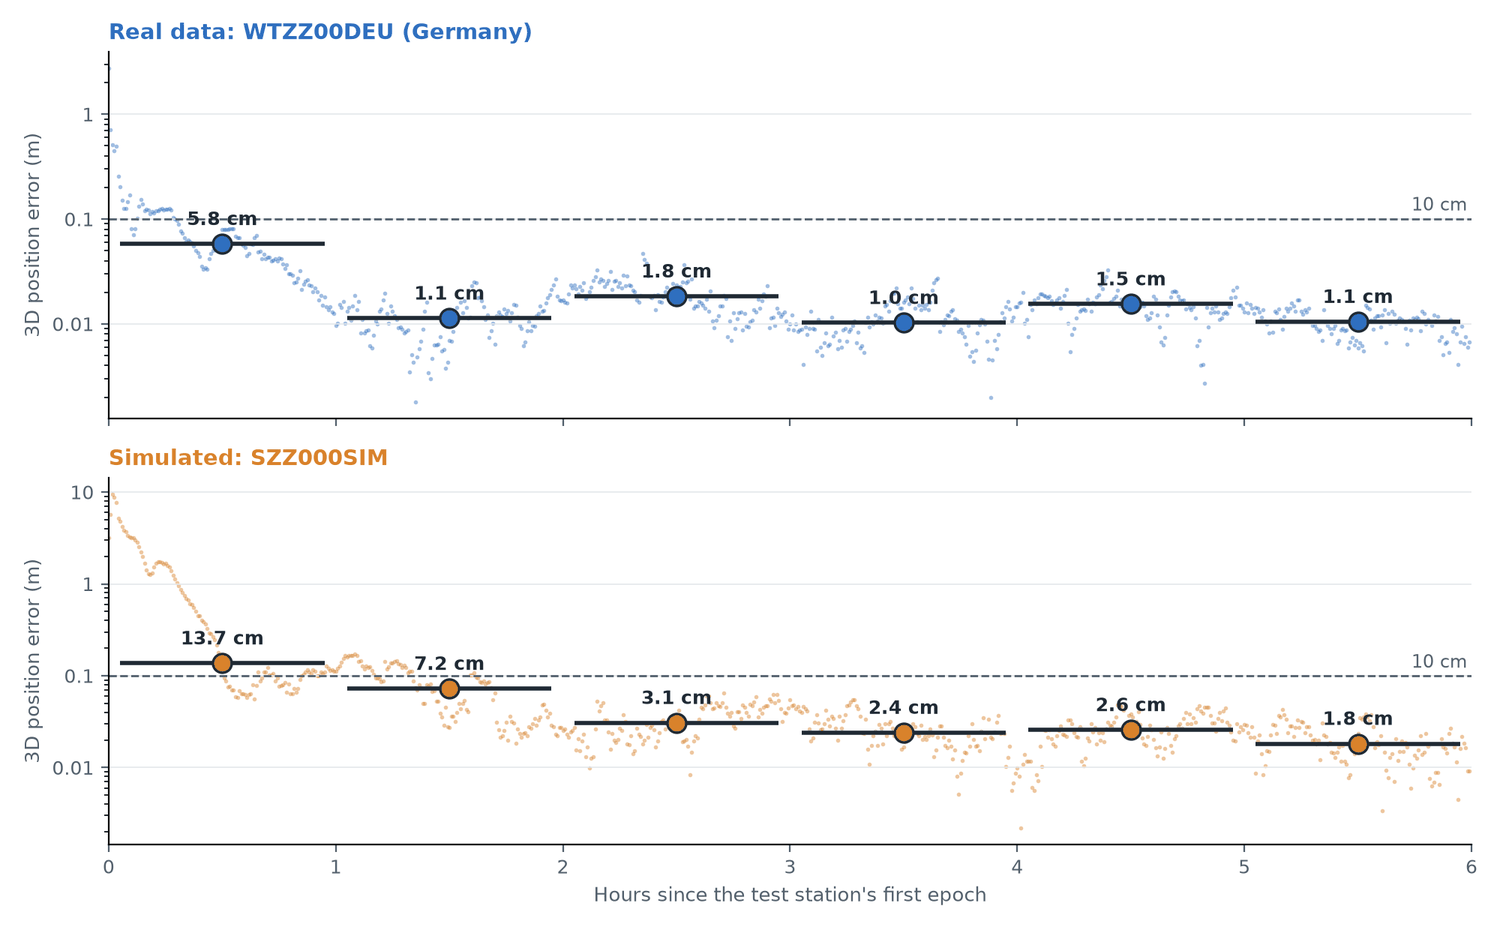
\includegraphics[width=0.5\linewidth]{test_station_by_hour.png}\hfill
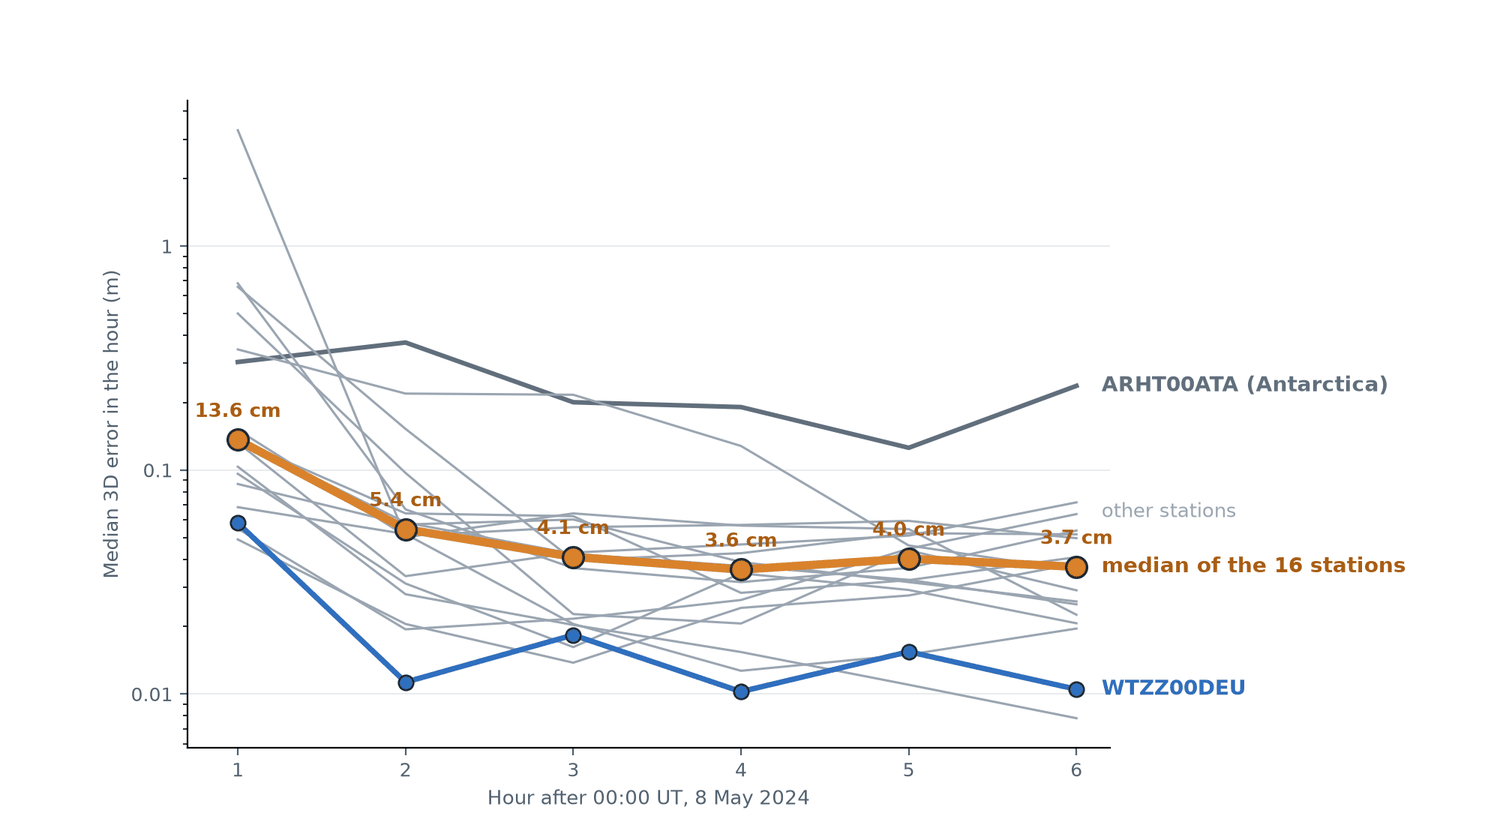
\includegraphics[width=0.48\linewidth]{sixteen_stations.png}
\caption{Left: the test station with our network's corrections, real data
(WTZZ00DEU, top) and simulated (SZZ000SIM, bottom); dots are epochs, bars hourly
medians. Right: hourly median for the 16 further stations (grey), their median
(orange), WTZZ00DEU (blue) and ARHT00ATA (dark). Status report figures.}
\label{fig:l9-a}
\end{figure}

\begin{figure}[h]
\centering
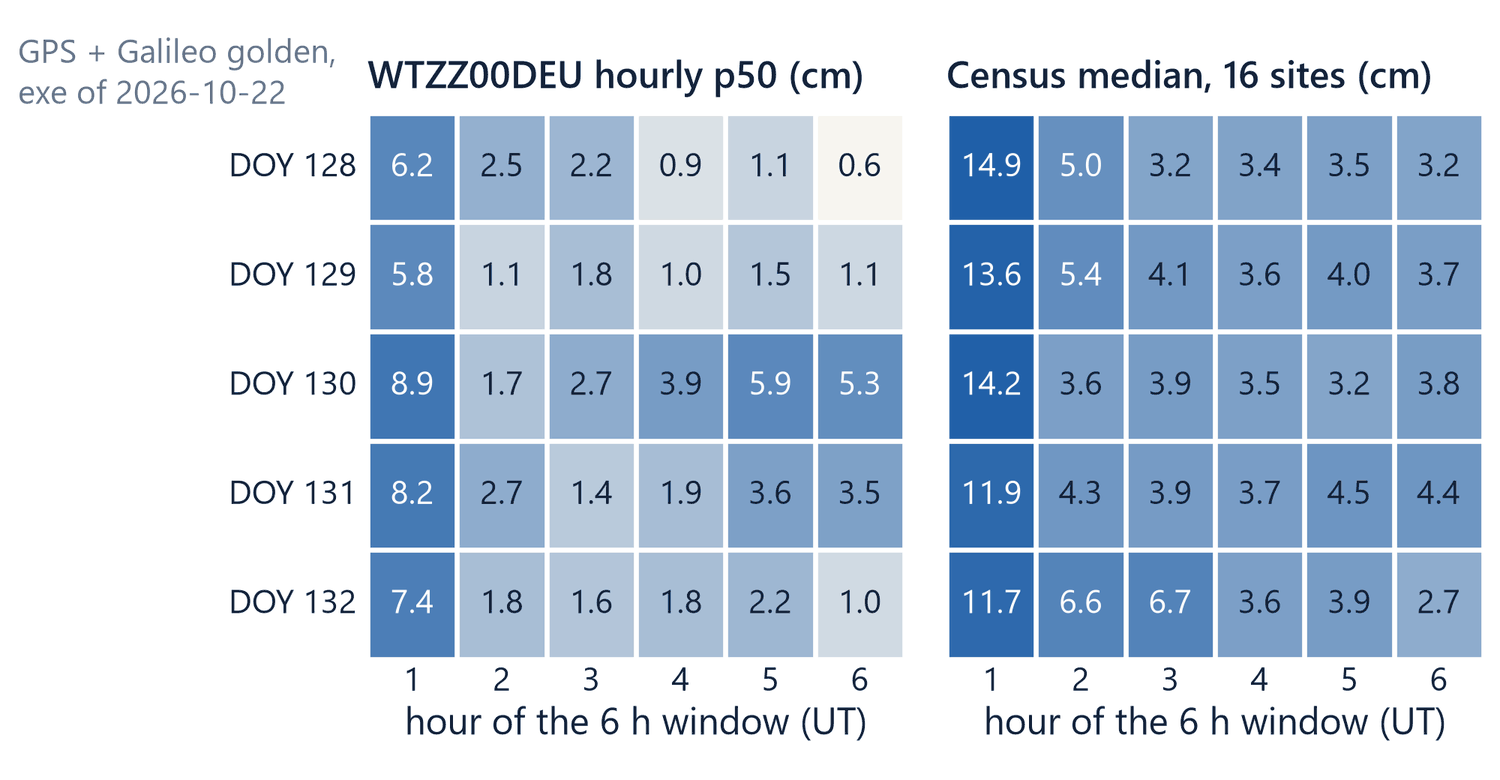
\includegraphics[width=0.52\linewidth]{five_days.png}\hfill
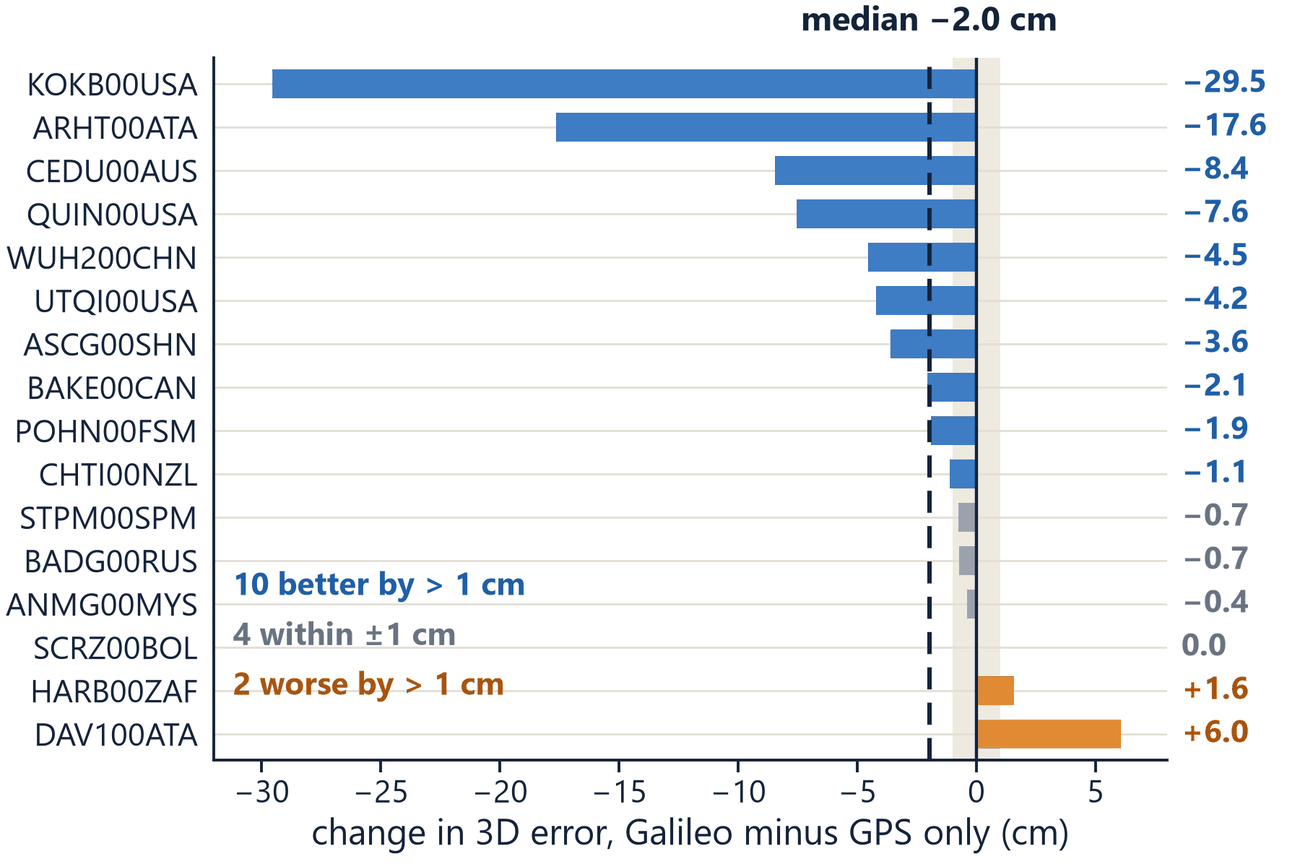
\includegraphics[width=0.46\linewidth]{galileo_change_per_station.png}
\caption{Left: five days, 7 to 11 May 2024, hourly median in cm: WTZZ00DEU and the
median of the 16 stations (the labels ``golden'' and ``census'' are the record's
names for the reference configuration and the 16 stations; deck slide 33). Right:
change of each station's error in hours 2 to 6 when Galileo is added, median
$-2.0$~cm (deck slide 19).}
\label{fig:l9-b}
\end{figure}

\begin{figure}[h]
\centering
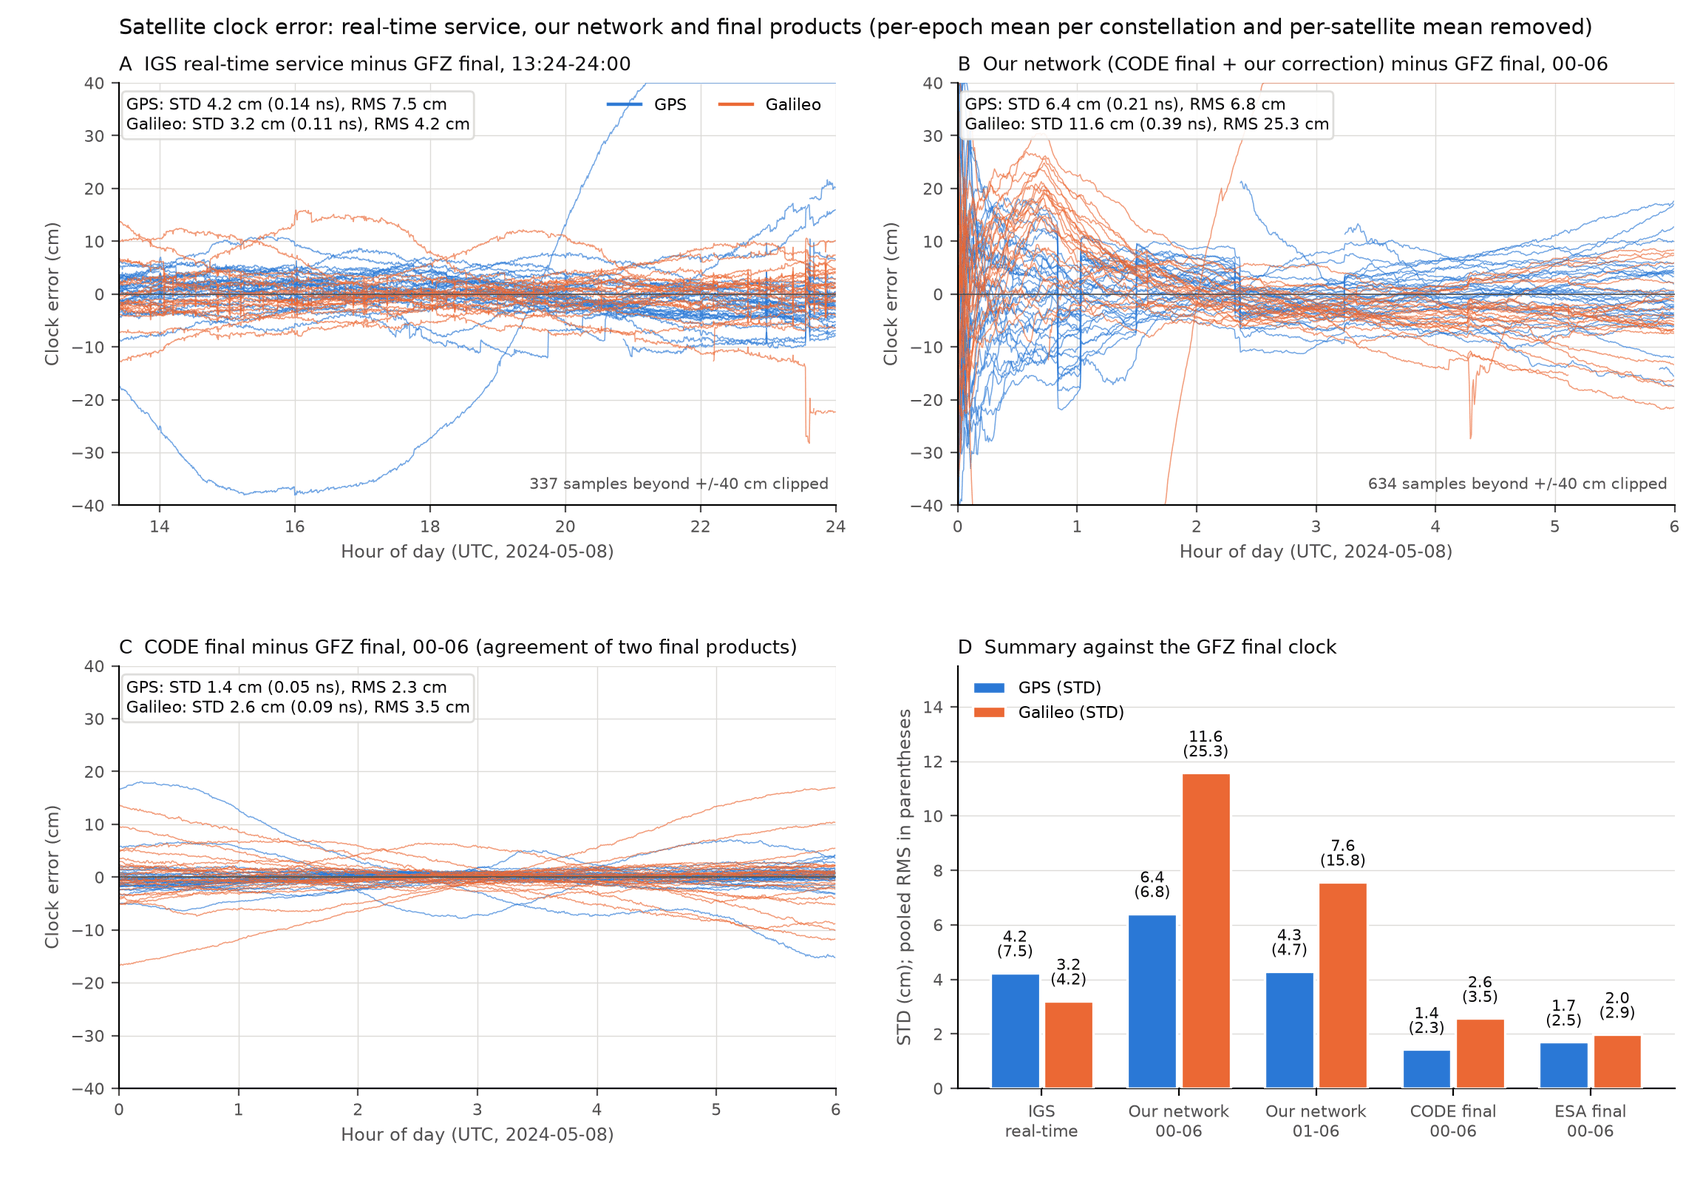
\includegraphics[width=0.62\linewidth]{clock_against_gfz.png}\hfill
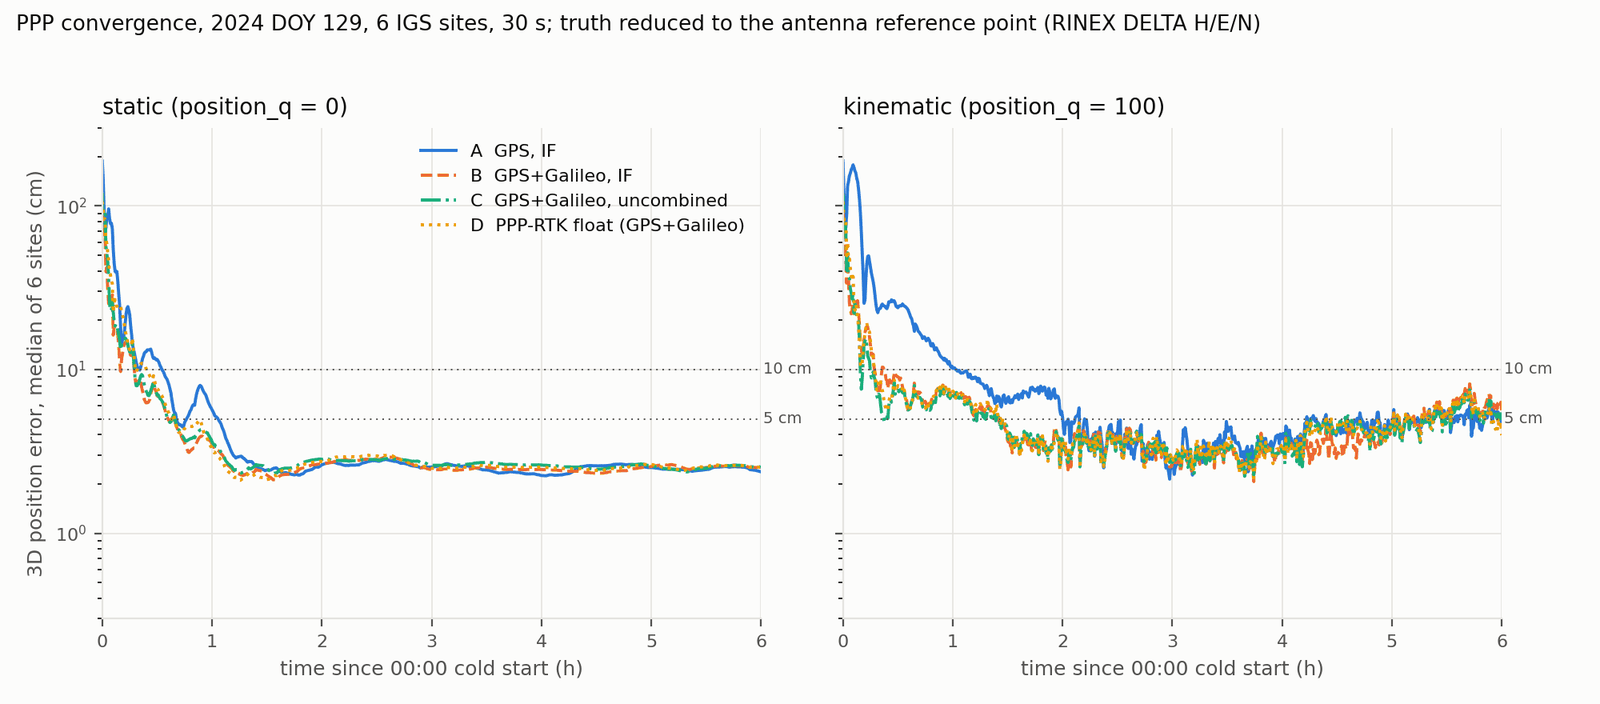
\includegraphics[width=0.36\linewidth]{ppp_convergence.png}
\caption{Left: satellite clock error against the GFZ final clock after removing the
per-system epoch mean and each satellite's mean: (A) IGS real-time service, (B) our
network, CODE final plus our correction, 00:00 to 06:00 with the first hour, (C)
CODE final, (D) summary (\texttt{results/t3/fig\_clock\_limits\_plain.png}). Right:
the PPP comparison of steps 1 to 3, median over six stations, static and moving
receiver (\texttt{results/t1/fig\_t1\_convergence.png}).}
\label{fig:l9-c}
\end{figure}

\begin{question}{census}{measure}{The test station and the 16 stations}{\ref{q:refsat}}
Run (about 2~s and 14~s):
\begin{cmd}
C:/Python313/python.exe scripts/rapid_arm.py score \
    runs/_rf0hv15_field6 runs/_rf0hv15_sim6
C:/Python313/python.exe scripts/clock_level/gcensus.py grade galpc galp galpg
\end{cmd}
Read the test station's median error by hour on both data sets, the 16 stations'
median by hour and the paired Galileo result. By what factor is hour 1 worse than
the mean of hours 2 to 6, at WTZZ00DEU and at the median station? In which mode is
WTZZ00DEU positioned (\texttt{runs/\_rf0hv15\_field6/arm.json}:
\texttt{filter.process\_noise.position\_q}, \texttt{network.closed\_loop.ar\_mode}),
and which network stations share its site?
\end{question}

\begin{question}{fivedays}{derive}{Five days from the stored grades}{\ref{q:census}}
\texttt{D:/GnssProcessorSupport/runs\_nom/mday\_galileo\_grades.txt} holds, per day
128 to 132, the 16 stations' median by hour and WTZZ00DEU by hour. From hours 2 to
6 of the five days, compute the median and the mean of the 25 sixteen-station
medians and the median of the 25 WTZZ00DEU values. On which day is WTZZ00DEU worse
than the median station in hours 4 to 6, and what does that do to ``the best
station''?
\end{question}

\begin{question}{t3}{read}{The clock against CODE and GFZ}{\ref{q:absorb} and \ref{q:hold}}
Read \texttt{results/t3/table\_clock\_report.tex} and \texttt{results/t3/results.md}
(the summary table and lines 100 to 113). Which clock is compared with which, over
which hours? Why is GFZ the reference and not CODE? Over the same hours, how does
the network's corrected clock compare with CODE's alone? What do the correlations
of the correction with (GFZ minus CODE) and (ESA minus CODE) say?
\end{question}

\begin{question}{capstone}{synthesis}{What the presentation may claim}{the whole course}
For each of five topics, state in two or three sentences what the presentation of
29~October may claim and the evidence that bounds it: (a) the model and its
per-epoch check; (b) the reference choices; (c) the satellite clock; (d) integer
ambiguities; (e) the simulated and real-data results.
\end{question}

\lessonbox{What this lesson establishes}{%
\begin{itemize}[leftmargin=*, itemsep=0pt, topsep=2pt]
\item On 8 May 2024 the test station reaches 1.0 to 1.8~cm and the median of the 16
      further stations 3.6 to 5.4~cm in hours 2 to 6, without integers.
\item Over five days the median station holds 3.8~cm; the test station is the best
      station on some days, not all, and shares its site with network stations.
\item The network's corrected clock is noisier than CODE's alone and carries no
      clock information: the user's precision is CODE's.
\end{itemize}}


\clearpage
% ==================================================================
\section*{Answers}
\addcontentsline{toc}{section}{Answers}
% ==================================================================
Each answer gives its source: the card and lines, the file and lines, or the
run. Where a command reproduces the answer, \emph{Check} gives it. Answers
marked \emph{checked} were reproduced on 24~October 2026 (the list is in the
last section). Cards named by a short name are files in \texttt{docs/refound/}:
ALD \texttt{ALD\_anchor\_level\_datum\_2026-10-23.md}, ARL
\texttt{ARL\_integer\_ambiguity\_ladder\_2026-10-09.md}, CTU
\texttt{CTU\_coupling\_time\_update\_2026-09-28.md}, FCFC
\texttt{FCFC\_fixed\_cycle\_ledger\_2026-10-11.md}, GAD
\texttt{GAD\_galileo\_adoption\_2026-10-13.md}, IRD
\texttt{IRD\_integer\_recovering\_datum\_2026-10-13.md}, LAH
\texttt{LAH\_level\_aware\_hold\_2026-09-29.md}, NBP
\texttt{NBP\_native\_broadcast\_clock\_posture\_2026-10-07.md}, R1D
\texttt{R1D\_station\_level\_datum\_2026-10-23.md}, SCB
\texttt{SCB\_sim\_clock\_error\_bed\_2026-10-24.md}, SCL
\texttt{SCL\_self\_contained\_clock\_level\_2026-10-03.md}. The S-system cards
\texttt{SBASIS-THEORY-E.md} and \texttt{SBASIS-CONTRACT.md} are in
\texttt{docs/cards/network-vehicle/}. ``The worked example'' is
\texttt{docs/report/network\_example.tex} (Mathematical Reference, ``Worked
example: estimability in a two-receiver network''). Status report sections are
cited by name; its wording was qualified on 24~October with the boundaries of
\cref{q:capstone}.

% ==================================================================
%  Answers to lessons 1 to 4.
% ==================================================================

\subsection*{Lesson 1: one receiver}

\begin{answer}{rx-clock}
\begin{enumerate}[leftmargin=*, itemsep=1pt]
\item Every code row contains $\sLight\,\mathrm{d}t_\rx + B_{\rx,\sigl}$ and every
      phase row $\sLight\,\mathrm{d}t_\rx + b_{\rx,\sigl}$; each sum gains
      $\delta - \delta = 0$. One receiver has one such direction.
\item $B_{\rx,1} = B_{\rx,\mathrm{IF}} + d_\rx$ and
      $B_{\rx,2} = B_{\rx,\mathrm{IF}} + \mu_2 d_\rx$ give
      $d_\rx = (B_{\rx,2} - B_{\rx,1})/(\mu_2 - 1)$ and
      $B_{\rx,\mathrm{IF}} = (\mu_2 B_{\rx,1} - B_{\rx,2})/(\mu_2 - 1)
      = (f_1^2 B_{\rx,1} - f_2^2 B_{\rx,2})/(f_1^2 - f_2^2)$, the ionosphere-free
      combination. $d_\rx$ is a scaled receiver DCB.
\item $\code^\sat_{\rx,\sigl} = \dots + (\sLight\,\mathrm{d}t_\rx + B_{\rx,\mathrm{IF}})
      + \mu_\sigl (I^\sat_\rx + d_\rx) + \dots$: the clock appears only as
      $\sLight\,\mathrm{d}t_\rx + B_{\rx,\mathrm{IF}}$. A user's ``receiver clock''
      is this ionosphere-free clock. The network defines the satellite clock the
      same way: ``the ionosphere-free clock (clock + IF code bias)''.
\end{enumerate}
\src{status report, ``One observation model''; \texttt{SBASIS-THEORY-E.md} lines 87
to 92 (the equations) and 158 to 160 (the ionosphere-free clock).}
\end{answer}

\begin{answer}{rx-phase}
\begin{enumerate}[leftmargin=*, itemsep=1pt]
\item $\lambda_\sigl (N + \delta_\sigl/\lambda_\sigl) + (b_{\rx,\sigl} - \delta_\sigl)
      = \lambda_\sigl N + b_{\rx,\sigl}$ for every satellite. One direction per
      signal: two for a dual-frequency receiver (type 4 of the network table, which
      counts $f(n-1)$ of them).
\item It estimates $N^\sat_{\rx,\sigl} + b_{\rx,\sigl}/\lambda_\sigl$ (and, without
      satellite phase biases, $-\,b^\sat_\sigl/\lambda_\sigl$ as well). The receiver
      phase bias is a fraction of a cycle common to all satellites, so the float
      ambiguity is not an integer however exact the satellite biases are. The same
      absorption makes ``a constant satellite phase bias simply join the
      ambiguity, so case D matches case C'' (status report, step 3).
\item The difference between two satellites removes $b_{\rx,\sigl}$, common to both.
      It is an integer only if both satellites' phase biases are removed exactly:
      the product must publish them (the observable-specific biases of step 3).
\end{enumerate}
\src{\texttt{SBASIS-THEORY-E.md} lines 97 to 104 (type 4); status report, step 3.}
\end{answer}

\begin{answer}{rx-iono}
\begin{enumerate}[leftmargin=*, itemsep=1pt]
\item $\mu_\sigl I^\sat_\rx + B_{\rx,\sigl} = B_{\rx,\mathrm{IF}} + \mu_\sigl(I^\sat_\rx + d_\rx)$.
\item On code, $\mu_\sigl(I + \delta + d - \delta)$ is unchanged. On phase the
      shifted ionosphere adds $-\mu_\sigl\delta$ to every satellite's row; the float
      ambiguities absorb it, $N^\sat_{\rx,\sigl} \to N^\sat_{\rx,\sigl} +
      \mu_\sigl\delta/\lambda_\sigl$ for every satellite. One more direction per
      receiver.
\item The estimated slant ionosphere is $I^\sat_\rx + d_\rx$ (and, with satellite
      terms from a product, minus that product's satellite geometry-free bias). It
      is the physical ionosphere only if $d_\rx$ is fixed by a convention, such as a
      zero-mean condition on the receivers' DCBs, or separated by a vertical
      ionosphere model. This is Odijk's $\tilde\iota = \iota + d_{\rx,\mathrm{GF}} -
      d^s_{\mathrm{GF}}$ (types 2b and 3b), and the reason for the network's
      zero-mean receiver DCB prior (\cref{sec:l4}).
\end{enumerate}
\src{\texttt{SBASIS-THEORY-E.md} lines 122 to 128.}
\end{answer}

\subsection*{Lesson 2: two receivers}

\begin{answer}{toy-normals}
\begin{enumerate}[leftmargin=*, itemsep=1pt]
\item Each code row has $+1$ in its receiver's column and $-1$ in its satellite's.
      $\bm{N} = \bm{A}^\Tr\bm{A}$ has 4 on the receiver diagonal (each receiver
      clock is in four rows), 2 on the satellite diagonal, $-1$ between every
      receiver and every satellite clock, and 0 elsewhere:
\[
\bm{N} = \begin{bmatrix} 4\bm{I}_2 & -\bm{J}_{2\times4} \\ -\bm{J}_{4\times2} & 2\bm{I}_4 \end{bmatrix},
\qquad \bm{J}\ \text{all ones.}
\]
\item Every row sums to zero ($4 - 4 = 0$; $-1 - 1 + 2 = 0$), so $\bm{N}\bm{1} =
      \bm{0}$; the rank is 5.
\item $\bm{1}$ adds the same $\kappa$ to every clock, receiver and satellite. Each
      observation is a difference $a_\rx - g^\sat$, so none changes, and no number of
      such observations fixes the common level: one reference choice is needed
      (type 1a). \emph{Checked.}
\end{enumerate}
\src{the worked example, eq.~ex-code-normals.}
\chk
\begin{cmd}
C:/Python313/python.exe - <<'EOF'
import numpy as np
A = np.array([[1 if j == r else 0 for j in range(2)]
              + [-1 if k == i else 0 for k in range(4)]
              for r in range(2) for i in range(4)])
N = A.T @ A
print(N, np.linalg.matrix_rank(N), N @ np.ones(6))
EOF
\end{cmd}
\end{answer}

\begin{answer}{toy-datums}
\begin{enumerate}[leftmargin=*, itemsep=1pt]
\item $a_A \equiv 0$: $g^\sat = -\code^\sat_A$, $a_B = a_A - (\code^1_A - \code^1_B)$:
      $a_B = -2$, $g = (-3, -6, -1, -4.5)$. $g^1 \equiv 0$: $a_A = \code^1_A = 3$,
      $a_B = \code^1_B = 1$, $g^\sat = a_A - \code^\sat_A = (0, -3, 2, -1.5)$.
\item The second minus the first is $3$ on every unknown: $3\cdot\bm{1}$, a vector of
      the null space.
\item $a_A - a_B = 2$, $g^2 - g^1 = -3$, $g^3 - g^1 = 2$, $a_B - g^4 = 2.5$ in both, and
      in the truth. Each combination $\bm{f}$ has $\bm{f}^\Tr\bm{1} = 0$, so adding
      a multiple of $\bm{1}$ cannot change it: the datum-invariance theorem in six
      unknowns (\cref{q:theorem}).
\item $\hat g^2 = g^2 - a_A = -1 - 5 = -6$: the true clock shifted by the reference
      receiver's clock. This lump is why a network declares its choice.
      \emph{Checked.}
\end{enumerate}
\src{the worked example, tables ``Two datum choices, same fit'' and ``What is
invariant''.}
\end{answer}

\begin{answer}{toy-phase}
\begin{enumerate}[leftmargin=*, itemsep=1pt]
\item Unknowns $6 + 4 + 8 = 18$; observations 16; null directions 5: the clock
      direction of \cref{q:toy-normals} and one per satellite,
      $(b^\sat + c_\sat,\ N^\sat_A - c_\sat,\ N^\sat_B - c_\sat)$; rank 13;
      redundancy $16 - 13 = 3$, the three code double differences
      ($(n-1)(m-1)$), identically zero in this noise-free model.
\item With $A$ alone each satellite's phase gives one equation in $b^\sat +
      N^\sat_A$: two unknowns that cannot be separated. With $B$ there are two
      equations in three unknowns, rank 2; the new estimable quantity is $N^\sat_A -
      N^\sat_B$, the between-receiver single difference.
\item With $a_A \equiv 0$, $a_A - g^\sat = \code^\sat_A$, so
      $\bar b^\sat = \phaseo^\sat_A - \code^\sat_A = (10.10, -5.20, 20.05, 8.15)$ and
      $\hat N^\sat_B = \phaseo^\sat_B - \code^\sat_B - \bar b^\sat = (2, 2, -2, 1)$.
\item $\bar b^1 = b^1 + N^1_A = 0.10 + 10$: the emitted bias carries the pinned
      receiver's ambiguity, Odijk's $\bar b^\sat = b^\sat + $ (pivot-receiver
      ambiguity). $\hat N^\sat_B = N^\sat_B - N^\sat_A$, the between-receiver single
      difference an RTK user fixes. \emph{Checked.}
\end{enumerate}
\src{the worked example, ``Adding carrier phase''.}
\end{answer}

\begin{answer}{toy-biases}
\begin{enumerate}[leftmargin=*, itemsep=1pt]
\item $1 + 2 + 1 + 4 + 1 + 4 = 13$, which is Eq.~24 with $f = 1$, $n = 2$, $m = 4$:
      $1 + 2 + 2(1 + 4) = 13$.
\item The full model has 26 unknowns (clocks 6, receiver and satellite code biases
      $2 + 4$, receiver phase biases 2, satellite phase biases 4, ambiguities 8);
      the lumped model 18. The lumps remove 8 unknowns ($B_\rx$, $B^\sat$, $b_\rx$)
      without changing the column space, so the rank stays 13 and the null space
      drops from $26 - 13 = 13$ to $18 - 13 = 5$. Gone: types 1b (2), 2a (1), 3a (4)
      and 4 (1), eight in all. Left: 1a (1) and 5 (4), the five of
      \cref{q:toy-phase}. A lump is itself a reference choice: defining $a_\rx =
      \sLight\,\mathrm{d}t_\rx + B_\rx$ fixes the split along the removed
      directions. \emph{Checked.}
\end{enumerate}
\src{\texttt{SBASIS-THEORY-E.md} lines 97 to 114 (the table and Eq.~24).}
\end{answer}

\begin{answer}{toy-user}
\begin{enumerate}[leftmargin=*, itemsep=1pt]
\item $\code^\sat_C = a_C - g^\sat = (2, 5, 0, 3.5)$;
      $\phaseo^\sat_C = a_C - g^\sat + b^\sat + N^\sat_C = (13.10, 0.80, 19.05, 13.65)$.
\item Code: $\hat a_C = \code^\sat_C + \hat g^\sat = -1$ for every satellite. Phase:
      $\tilde N^\sat_C = \phaseo^\sat_C - \hat a_C + \hat g^\sat - \bar b^\sat = (1, 1,
      -1, 2)$.
\item $\hat a_C = a_C - a_A = 4 - 5$, through $\hat g^\sat = g^\sat - a_A$;
      $\tilde N^\sat_C = N^\sat_C - N^\sat_A$, through $\bar b^\sat = b^\sat +
      N^\sat_A$. $C$'s solution carries receiver $A$'s clock and ambiguities, and $C$
      needs no knowledge of $A$: ``the user never needs to know the network
      pivot'', and PPP-RTK is relative positioning. \emph{Checked.}
\end{enumerate}
\src{\texttt{SBASIS-THEORY-E.md} lines 166 to 170.}
\end{answer}

\begin{answer}{toy-setchange}
\begin{enumerate}[leftmargin=*, itemsep=1pt]
\item $\sum g^\sat = -2.5$ under $g^1 \equiv 0$; adding $\kappa = 0.625$ to every
      clock gives $g = (0.625,\allowbreak -2.375,\allowbreak 2.625,\allowbreak -0.875)$
      and $a = (3.625, 1.625)$.
\item Pin: $g = (0, -3, 2)$, $a = (3, 1)$; nothing moves. Sum-to-zero over
      satellites 1 to 3: $\kappa = 1/3$, $g = (0.333, -2.667, 2.333)$,
      $a = (3.333, 1.333)$: every clock moves by $-0.292$~m.
\item The pin moves to satellite 2: every clock moves by $+3$~m (the old $\hat
      g^2 = -3$): $g = (\cdot, 0, 5, 1.5)$, $a = (6, 4)$.
\item None: every move is along $\bm{1}$, so all differences stay. A user absorbs
      the common step in its receiver clock at that epoch, but any state it carries
      across the epoch at the old level sees a step, so the step must be declared
      and the user resets across it. Sum-to-zero ``steps at every
      constellation-membership change''; a pin moves only when its own satellite
      leaves, a handover the consumer ``pays for with an ambiguity reset''. The
      project uses a pin with a sticky pivot and declares each handover
      (\cref{q:step}). \emph{Checked.}
\end{enumerate}
\src{\texttt{SBASIS-THEORY-E.md} line 145; \texttt{include/network/solve/Sbasis.hpp}
lines 162 to 166.}
\end{answer}

\subsection*{Lesson 3: the real network}

\begin{answer}{schur}
\begin{enumerate}[leftmargin=*, itemsep=1pt]
\item $\bm{N}_{aa} = 4\bm{I}_2$, $\bm{N}_{ag} = -\bm{J}$, so
      $\bm{N}_{ga}\bm{N}_{aa}^{-1}\bm{N}_{ag} = \tfrac{2}{4}\bm{J}_4$ and
      $\bar{\bm{N}}_{gg} = 2\bm{I}_4 - 0.5\,\bm{J}_4$ (1.5 on the diagonal, $-0.5$ off
      it). With $\bm{u}_a = (14.5, 6.5)$ (the sums of each receiver's pseudoranges)
      and $\bm{u}_g = -(4, 10, 0, 7)$: $\bar{\bm{u}}_g = \bm{u}_g + (14.5 + 6.5)/4 =
      (1.25, -4.75, 5.25, -1.75)$. It sums to zero: the data are consistent along
      the null direction.
\item $\bm{J}_4$ has eigenvalues 4 (along $\bm{1}$) and 0 (three times), so
      $\bar{\bm{N}}_{gg}$ has 0 (along $\bm{1}$) and 2 (three times). The null
      eigenvector is $(0.5, 0.5, 0.5, 0.5)$: weight $1/\sqrt{4}$ on every satellite
      clock, the clock direction of \cref{q:toy-normals} seen from the satellites.
\item The rows read $2g^\sat - 0.5\,S = \bar u_\sat$ with $S = \sum g^\sat$. With
      $g^1 = 0$: $S = -2.5$, $g = (0, -3, 2, -1.5)$. Back-substitution
      $a_\rx = (u_{a,\rx} + S)/4$ gives $a = (3, 1)$, the solution of
      \cref{q:toy-datums}: the elimination is exact. \emph{Checked.}
\end{enumerate}
\src{\cref{eq:l3-schur} (status report, step 6); the worked example's data.}
\end{answer}

\begin{answer}{twosys}
\begin{enumerate}[leftmargin=*, itemsep=1pt]
\item Two. The GPS clock direction: every receiver clock and every satellite clock,
      GPS and Galileo, $+\kappa$ (each Galileo row holds $a_\rx - g^\sat$ too). The
      Galileo direction: $d^E_\rx + \kappa_E$ at every receiver and $g^\sat +
      \kappa_E$ for every Galileo satellite.
\item Two, spanned by a flat shift of the GPS clocks and a flat shift of the
      Galileo clocks; the receiver terms are gone. When both eigenvalues are zero an
      eigensolver may return any rotation of the pair.
\item $1/\sqrt{32} = 0.1768$ on every GPS clock and $1/\sqrt{24} = 0.2041$ on every
      Galileo clock. A small check (two receivers, three GPS and two Galileo
      satellites) has 9 unknowns, rank 7 and a two-dimensional reduced null space
      constant within each constellation. \emph{Checked.}
\end{enumerate}
\src{the arithmetic; the real run in \cref{q:rankgate}.}
\end{answer}

\begin{answer}{eq24}
\begin{enumerate}[leftmargin=*, itemsep=1pt]
\item $1 + 2f + (n-1) + m + f(n-1) + f\,m = 1 + 2f + (1+f)(n-1+m)$; with the slant
      ionosphere $+\,(n - 1 + m)$.
\item $f = 2$, $m = 32$: $5 + 3(n + 31) + (n + 31) = 5 + 4(n + 31)$, which gives 369
      for $n = 60$, 361 for 58 and 1,349 for 305. The slope 4 per station is the
      figure's ``slant ionosphere: 4 per station''; without the slant term it is 3.
\item $1 + 4 + 3 \times 115 = 350$, plus 115: 465. Eq.~24 is a single-system count
      and the record has no two-system form, so 465 sets the scale only.
      \emph{Checked.}
\end{enumerate}
\src{\texttt{SBASIS-THEORY-E.md} lines 106 to 114; deck slide 6.}
\chk
\begin{cmd}
C:/Python313/python.exe - <<'EOF'
f = 2
for n, m in ((60, 32), (58, 32), (305, 32), (60, 56)):
    print(n, m, 1 + 2*f + (1 + f)*(n - 1 + m) + (n - 1 + m))
EOF
\end{cmd}
\end{answer}

\begin{answer}{inventory}
\begin{enumerate}[leftmargin=*, itemsep=1pt]
\item Shared: satellite clock (GPS, Galileo), satellite phase bias (GPS L1C, L2W;
      Galileo L1C, L5Q), satellite code bias (GPS C1C, C2W; Galileo C1C, C5Q); the
      counts (498, 393) are station-held instances, one per line of sight. Local:
      ambiguity per signal, slant ionosphere per system, zenith wet delay (60),
      receiver clock (60), Galileo inter-system bias (60), receiver DCB per system;
      receiver position 180 columns ``pinned: held at the roster coordinate''.
      $\mathrm{d}t_\rx \to$ receiver clock, $\delta t_\rx$ $\to$ inter-system bias,
      $T \to$ zenith wet delay, $I \to$ slant ionosphere, $B_{\rx,\sigl} \to$
      receiver DCB, $N \to$ ambiguity; the satellite terms $\to$ the shared rows.
      The receiver phase bias has no row (the parameter-model line reads
      \texttt{rx\_phase\_bias no no}, line 380): the ambiguities absorb it, as in
      \cref{q:rx-phase}.
\item Shared $(1 + 2f)\,m = 5 \times 56 = 280$ (line 639, \texttt{nshared=280}).
      Local: 3 per line of sight (two ambiguities, one slant ionosphere) $\times$
      891 lines of sight, plus 5 per station $\times$ 60: $2{,}673 + 300 = 2{,}973$.
      \emph{Checked.}
\end{enumerate}
\src{\texttt{runs/\_rf0hv15\_sim6/stdout.txt} lines 380, 639, 658 to 686;
\texttt{src/core/network/assembly/ParamInventory.cpp} lines 645 to 661.}
\end{answer}

\begin{answer}{rankgate}
\begin{enumerate}[leftmargin=*, itemsep=1pt]
\item At tow 259230: $+4.036\times10^{-11}$ and $-1.803\times10^{-10}$ (a negative
      value is a rounded zero), with weights 0.2040 on every Galileo clock and
      0.1767 on every GPS clock: exactly the flat shifts of \cref{q:twosys}.
\item Cutoff $= 10^{-11}\times1.0459\times10^5 = 1.0459\times10^{-6}$; cutoff$/1.803
      \times10^{-10} = 5.8\times10^3$ (3.8 decades); the weakest real direction,
      $1.124\times10^{-4}$ (a GPS L2W phase-bias direction), is 107 times the cutoff
      (2.0 decades). The rule, ``cutoff $\geq$ 2 decades above the gauge depth and
      $\geq$ 2 decades below the weakest-real layer'', holds, the upper margin only
      just. The run end (line 4899) reports 720 epochs at tol $10^{-11}$, 720
      emitted, none withheld, observed count min 2, max 2.
\item Lumps and rows remove them before the gate, as in \cref{q:toy-biases}. The
      record maps the types to rows: 1a to the 2 clock pins (acting after the
      gate); 3a and 3b to 112 code-bias rows; 5 to 112 ambiguity pins; 1b, 2a, 2b and
      4 (240) to the receiver side, which is local (free clock, inter-system bias,
      DCB with 120 prior entries, no receiver phase-bias state). $2 + 112 + 112 +
      240 = 466 = 465 + 1$, the extra one being the second constellation's clock
      direction. \emph{Checked.}
\end{enumerate}
\src{\texttt{rf\_null\_space\_read.py} output; \texttt{runs/\_rf0hv15\_sim6/logs/network\_estimability.csv}
rows 2 to 6; \texttt{runs/\_rf0hv15\_sim6/stdout.txt} lines 640, 4899;
\texttt{RankGate.cpp} lines 408 to 410; \texttt{SBASIS-CONTRACT.md} lines 59 to 68.}
\end{answer}

\subsection*{Lesson 4: the project's reference choices}

\begin{answer}{theorem}
\begin{enumerate}[leftmargin=*, itemsep=1pt]
\item An estimable function $\bm{f}^\Tr\bm{x}$ ($\bm{f}$ in the range of
      $\bm{A}^\Tr$) ``is invariant in value AND variance under any admissible
      datum'', that is, under every reference choice that removes exactly the null
      space. \Cref{q:toy-datums} showed the value half: four differences equal in
      two choices.
\item Position, zenith delay and vertical ionosphere are estimable before any choice
      (their rows of the null-space basis are zero). A satellite clock and a
      satellite phase bias are not: ``The satellite clock does not exist as an
      estimable number; only a datum-dependent lump does.''
\item The differential wander was estimable, so no reference choice could move it,
      and every datum comparison came out negative: ``The cure must alter
      ESTIMATION (weights / dynamics / model / transmitted covariance), not the
      gauge.'' The coverage change that cut the wander from 47 to 14~cm was such a
      change.
\end{enumerate}
\src{\texttt{SBASIS-THEORY-E.md} lines 40 to 41, 75 to 83, 116 to 120, 223 to 225.}
\chk
\begin{cmd}
sed -n '75,83p;116,120p' docs/cards/network-vehicle/SBASIS-THEORY-E.md
\end{cmd}
\end{answer}

\begin{answer}{four}
The verify prints, per reference configuration, ``76 recommended knobs armed in
regime, 2 unarmed (2 documented exceptions), 0 failure(s)'' and ``golden verify:
PASS''. \emph{Checked.}
\begin{enumerate}[leftmargin=*, itemsep=1pt]
\item Clock pin: no key (the default), with \texttt{sticky\_pivot} (line 324) and
      \texttt{handover\_stransform} (343). Anchors: \texttt{phase\_datum\_prioritized}
      (297), \texttt{phase\_datum\_held\_basis} (925), \texttt{ambiguity\_vehicle}
      \texttt{float\_kf} (924). Code-bias datum: \texttt{estimate\_sat\_code\_bias}
      (293), \texttt{sat\_gf\_datum} \texttt{broadcast\_tgd} (922); the
      ionosphere-free pin and sum-to-zero rows have no key of their own. Receiver
      DCB prior: \texttt{rx\_code\_bias\_datum} (292).
\item The pin is unaffected by satellites rising and setting until the pivot
      leaves; then the constellation is re-referenced (one handover per
      constellation in 6~h: E02 to E03, G01 to G02). An anchor is a single point of
      failure: a handover steps the bias by whole cycles unless the successor is
      pinned at its own level (308 basis values elected, 22 of them cold, declared).
      The sum-to-zero rows would move at every rise and set, as in
      \cref{q:toy-setchange}; the simulated case suppresses them because the pins
      already fix every channel (2,880 suppressed $= 4 \times 720$). The ensemble was
      ``SUPERSEDED BY MEASUREMENT'' and deleted (commit 7914263).
\item \texttt{clock\_datum\_sum\_to\_zero}, \texttt{clock\_datum\_broadcast\_anchored},
      \texttt{pivot\_election}; \texttt{phase\_datum\_eq34} is false (line 345).
\end{enumerate}
\src{\texttt{SBASIS-THEORY-E.md} lines 143 to 150, 239 to 259; \texttt{Sbasis.hpp}
lines 162 to 166; \texttt{config/golden/golden\_sim\_refound.json}; \texttt{\_rap\_scb\_g\_q6/stdout.txt}
lines 4385, 4400, 4845.}
\chk
\begin{cmd}
C:/Python313/python.exe scripts/make_golden_config.py --verify
grep -n -e '"sticky_pivot"' -e '"phase_datum_held_basis"' -e '"phase_datum_eq34"' \
    config/golden/golden_sim_refound.json
\end{cmd}
\end{answer}

\begin{answer}{rows}
\begin{enumerate}[leftmargin=*, itemsep=1pt]
\item $56\times(1 + 2 + 2) = 280$ shared columns. Clock pins 2 (E02, G01). Ambiguity
      pins $112 = 32\times2 + 24\times2$, one per phase-bias column, on 18 stations.
      Code-bias rows 112: 56 ionosphere-free pins and 56 geometry-free pins at
      $T_{GD}$ (54 at $c\,T_{GD}$, 2 with a broadcast $T_{GD}$ of 0); sum-to-zero 0.
      Receiver prior entries $120 = 60\times2$, each of information $1/(10~\mathrm{m})^2
      = 0.01~\mathrm{m}^{-2}$. Total: 226 rows on the shared state plus 120 prior
      entries.
\item The ambiguity pins and code-bias rows act before the gate and fix the 224
      phase-bias and code-bias columns; the 56 clocks keep one flat direction per
      constellation (\cref{q:twosys}); the clock pins act in the solve after the
      gate, so the gate expects 2 (\texttt{Sbasis.hpp} lines 50 to 55: ``exactly
      \#constellations residual deficiencies'').
\item On a mismatch the gate throws; the heal soft-anchors near-null phase-bias
      columns ($\sigma$ 1~m) and re-gates once; if the count still differs the epoch is
      withheld and counted as under- or over-specified. Completion would first fold
      one eigenvector row per extra separable near-null direction; it folded none in
      720 epochs (line 4112). \emph{Checked.}
\end{enumerate}
\src{\texttt{\_rap\_scb\_g\_q6/stdout.txt} lines 631, 679 to 738, 4109, 4112, 4387;
\texttt{Sbasis.hpp} lines 50 to 55; \texttt{src/core/network/solve/RankGate.cpp}
lines 193 to 305.}
\chk
\begin{cmd}
sed -n '631p;679,738p;4109,4112p' \
    D:/GnssProcessorSupport/runs_nom/_rap_scb_g_q6/stdout.txt
\end{cmd}
\end{answer}

\begin{answer}{cbdatum}
\begin{enumerate}[leftmargin=*, itemsep=1pt]
\item \texttt{B,G05,C1C,-3.2108400641001413} and \texttt{B,G05,C2W,-5.288075205569585}:
      the ratio is $1.646944 = \mu_2$, so the ionosphere-free combination is zero.
      The navigation record gives $T_{GD} = -1.071020960808\times10^{-8}$~s, and
      $c\,T_{GD} = -3.2108400641$~m, the C1C record. The pinned pair carries no
      estimate: its ionosphere-free part is pinned to zero and its geometry-free
      part to the broadcast group delay (54 satellites at $c\,T_{GD}$, 2 with a
      broadcast value of 0; stdout line 631).
\item With a slant ionosphere the satellite's true geometry-free code bias is not
      estimable: it merges into the slant ionosphere of every line of sight to that
      satellite (\cref{q:rx-iono}, mirrored at the satellite). The corrections carry
      no ionosphere record, so a user estimates its own slant ionosphere, which
      absorbs the same lump: code biases and ionosphere act as a pair.
      \emph{Checked.}
\end{enumerate}
\src{\texttt{\_rap\_scb\_g\_q6/products.txt} lines 61 to 62;
\texttt{data/2024-129/products/BRDC00IGS\_R\_20241290000\_01D\_MN.rnx} line 568;
\texttt{docs/refound/RF-0c\_gf\_pin\_2026-09-15.md} lines 22 to 23;
\texttt{SBASIS-CONTRACT.md} lines 114 to 133.}
\chk
\begin{cmd}
C:/Python313/python.exe - <<'EOF'
print(299792458 * -1.071020960808e-08)          # c * T_GD of G05, m
print(-5.288075205569585 / -3.2108400641001413)  # C2W / C1C
print((1575.42 / 1227.60) ** 2)                 # mu_2
EOF
\end{cmd}
\end{answer}

\begin{answer}{level}
\begin{enumerate}[leftmargin=*, itemsep=1pt]
\item $0.0074/10^2 = 7.4\times10^{-5}~\mathrm{m}^{-2}$ along the unit level;
      $\sigma = 1/\sqrt{7.4\times10^{-5}} = 116$~m.
\item $(0.0074 + 0.2392^2 + 0.1334^2)/0.0074 = (0.0074 + 0.0572 + 0.0178)/0.0074 =
      11.1$, $\sigma$ about 35~m, still useless: card R1D found such a row changes
      nothing at 10~m, and at 1~m shrinks the move only by a fifth while pushing
      0.95~m into C1W rows: ``the datum row is not the fix''.
\item $\sigma = 1/\sqrt{110} = 0.095$~m. The carried ambiguity coupling supplies 109
      of the 110, the DCB prior $7\times10^{-5}$: the coupling to the shared state
      holds the level, not the datum.
\item The direction lives inside one station's block, which is eliminated before the
      shared matrix is formed (\cref{q:schur}), so the gate never sees it.
      MAJU00MHL anchored phase biases of five GPS satellites (13 pins). With the
      pins held, the station's level plus a matching shift of its anchored phase
      biases is invisible to its data (residual $2.8\times10^{-11}$), so a move of
      the level reaches the published phase biases. In the GPS L5 event the level
      moved $-21.92$~m; barring the station from the anchor election removed the
      event: ``The anchor loop is the transmission''. The hold card ALD derives is
      not built; GPS L5 stays sequenced.
\end{enumerate}
\src{card R1D lines 21 to 28, 54, 66 to 89, 99 to 122, 159; card ALD lines 27, 31 to 41,
54, 58 to 65.}
\chk
\begin{cmd}
C:/Python313/python.exe - <<'EOF'
import math
print(1 / math.sqrt(0.0074 / 100))                   # sigma from the prior, m
print((0.0074 + 0.2392**2 + 0.1334**2) / 0.0074)      # information factor
print(1 / math.sqrt(110))                            # sigma from the coupling, m
EOF
\end{cmd}
\end{answer}

% ==================================================================
%  Answers to lessons 5 to 9.
% ==================================================================

\subsection*{Lesson 5: what a user sees}

\begin{answer}{absorb}
\begin{enumerate}[leftmargin=*, itemsep=1pt]
\item $\Delta$ enters every code and phase row of system $g$ identically; the
      receiver clock (with the inter-system bias for a second system) takes it up,
      as $\hat a_C$ took up $a_A$ in \cref{q:toy-user}. The geometry, hence the
      position, is unchanged.
\item A constant $d$ enters only that satellite's phase rows, as a constant: the
      float ambiguity moves, $N \to N + d/\lambda$. The position is unchanged; only
      the ambiguity's meaning changes, which matters once a user fixes integers.
\item $(\delta, \mu_2\delta)$ adds $\mu_\sigl\delta$ to code row $\sigl$, the
      ionosphere's own signature, so $I^\sat \to I^\sat + \delta$ absorbs it; on
      phase that shift enters as $-\mu_\sigl\delta$, which the float ambiguities
      absorb. The position is unchanged; the user's slant ionosphere is biased by
      $\delta$. The ionosphere-free combination of $(\delta, \mu_2\delta)$ is zero, so
      an ionosphere-free user sees nothing at all.
\item The per-system mean at each epoch (case 1, the receiver clock), then each
      satellite's mean over the session (case 2, the ambiguity). Case 3 does not
      arise for clocks. The S-system statement: the user uses only the
      block-diagonal part of the correction covariance, ``the rank-one $[e;e]$
      (clock/geometry) and $[-\mu;\mu]$ (iono) parts lie in the user's own design
      range and are absorbed''.
\end{enumerate}
\src{\texttt{SBASIS-THEORY-E.md} lines 158 to 182; \texttt{SBASIS-CONTRACT.md}
lines 98 to 102, 114 to 133; status report, step 5; \texttt{results/t3/results.md}
lines 64 to 66.}
\end{answer}

\begin{answer}{sline}
\begin{center}\footnotesize
\begin{tabular}{@{}p{4.6cm}p{5.4cm}p{4.8cm}@{}}
\toprule
Field & Declares & Defined or written at \\
\midrule
\texttt{S30000SIM} & the run's reference (clock-datum) station; the pins act on satellite clocks & \texttt{ApplicationNetworkSetup.cpp} line 1485 \\
\texttt{1}, \texttt{nominal-wu93} & bias sign convention; phase wind-up model & \texttt{Sbasis.hpp} lines 98 to 108, 215 \\
\texttt{0} (5th field) & ambiguity datum: ``legacy single pivot and prioritized anchor'' & \texttt{Sbasis.hpp} lines 129 to 132 \\
\texttt{0} (6th field) & clock datum: one hard satellite clock pin per constellation & \texttt{Sbasis.hpp} lines 162 to 166 \\
\texttt{1}, \texttt{0} & the network emits its own code biases; code-bias datum id & \texttt{Sbasis.hpp} lines 229, 238 \\
\texttt{0.05}, \texttt{1} & clock discontinuity threshold (m); discontinuities emitted & \texttt{NetworkProductEmitter.hpp} lines 195 to 207 \\
the SP3 and CLK names & the a priori orbit and clock; every C record corrects this clock & \texttt{ApplicationNetworkSetup.cpp} lines 1524 to 1566 \\
\texttt{E:E02}, \texttt{G:G01} & realized clock pivots (C $= 0$ at the first epoch) & \texttt{SolPrep.cpp} lines 1176 to 1179 \\
\texttt{cbjump}, \texttt{atx}, \texttt{oref} & code-bias jump test; antenna file; orbits at the centre of mass & \texttt{NetworkProductEmitter.hpp} lines 222 to 228; \texttt{NetworkProductIO.hpp} lines 270 to 273 \\
\texttt{discfrac}, \texttt{hsig} & phase jump gate of 0.25 cycle; $\sigma_0$ of the H records & \texttt{NetworkProductEmitter.hpp} lines 238 to 248; \texttt{NetworkProductIO.hpp} lines 238 to 247 \\
\texttt{cbpin=...} & the ionosphere-free pin pair per system & \texttt{SolPrep.cpp} lines 1118 to 1157 \\
\texttt{sat\_gf\_datum=broadcast\_tgd} & the geometry-free datum at $c\,T_{GD}$ & \texttt{SolPrep.cpp} lines 1165 to 1172 \\
\texttt{pbhold=2} & the phase-clock hold (\cref{q:hold}) & \texttt{ApplicationNetworkSetup.cpp} lines 1599 to 1601 \\
\bottomrule
\end{tabular}
\end{center}
The reference choices of \cref{sec:l4} are the two datum ids, the pivots, the
\texttt{cbpin} pairs and \texttt{sat\_gf\_datum}; \texttt{pbhold} declares how the
phase biases are held. A current run appends \texttt{wumode=accumulated}. The
real-data S line declares only \texttt{cbpin=G:C1C-C2W}: the Galileo pairs are
``NOT declared (per-satellite split)'' (\texttt{runs/\_rf0hv15\_field6/stdout.txt}
line 686).
\src{\texttt{src/core/products/NetworkProductIO.cpp} lines 465 to 602 and the lines
in the table (paths under \texttt{src/core/network/} and \texttt{include/}).}
\chk
\begin{cmd}
sed -n '2p' D:/GnssProcessorSupport/runs_nom/_rap_scb_g_q6/products.txt
\end{cmd}
\end{answer}

\begin{answer}{step}
\begin{enumerate}[leftmargin=*, itemsep=1pt]
\item The awk prints line 134213, \texttt{E,2313,271230.00000715256,400,0,0,1,E}
      (Galileo, 03:20:30), and line 189631, \texttt{E,2313,276149.99999547005,564,0,0,1,G}
      (GPS, 04:42:30). The script prints ``31 satellites, mean step 1.6278 m, sd
      after the mean 0.0027 m''; an ordinary pair of epochs (276090 to 276120) gives
      $-0.0001$ and 0.0008~m.
\item The handover of \cref{q:toy-setchange} (3): the pivot moved from G01 to G02 and
      every GPS clock stepped by the old pivot-relative value. A user's receiver
      clock absorbs the common 1.63~m; 3~mm per satellite stays visible.
\item A raw-step grade sees 31 satellites jump 1.6~m at once; the datum-invariant
      step is 3~mm. On real data the GPS group mean steps by about $+154$~cm at its
      pivot change. \emph{Checked.}
\end{enumerate}
\src{\texttt{runs/\_rf0hv15\_sim6/products.txt}; \texttt{results/t3/results.md}
lines 105 to 107.}
\end{answer}

\begin{answer}{refsat}
\begin{enumerate}[leftmargin=*, itemsep=1pt]
\item A chord is $e_\sat = s_\sat - s_{\mathrm{ref}}$: $\mathrm{Var}(e_\sat) =
      \sigma^2 + \sigma_{\mathrm{ref}}^2$ and $\mathrm{Cov}(e_\sat, e_k) =
      \sigma_{\mathrm{ref}}^2$, so two chords correlate by
      $\sigma_{\mathrm{ref}}^2/(\sigma^2 + \sigma_{\mathrm{ref}}^2)$, 0.5 when
      $\sigma_{\mathrm{ref}} = \sigma$.
\item L1C over all epochs: as traced, median $|e|$ 0.304 cycle, 65.3\,\% round to
      the right integer; reference-free 0.122 cycle, 81.6\,\%. Last quarter: 0.260
      cycle and 69.5\,\% against 0.092 cycle and 86.5\,\%.
\item The reference satellite's error and its returns enter every chord, so a grade
      on the traced chords reports that one element's share: ``Quote DD grades
      ref-free from now on.'' A second trap of the same card: subtracting a group's
      own circular median shrinks uniform noise from 0.251 to 0.145 cycle, so a
      wrapped grade is quoted as a gap to a size-matched null. \emph{Checked.}
\end{enumerate}
\src{\texttt{docs/cards/sim-bed/DD-TRACE-REF-SAT.md} lines 41 to 48, 107 to 110, 143
to 159; \texttt{CLAUDE.md}, ``Grading traps that still apply''.}
\end{answer}

\subsection*{Lesson 6: the satellite clock}

\begin{answer}{qstep}
\begin{enumerate}[leftmargin=*, itemsep=1pt]
\item $\sqrt{2.9\times10^{-8}\times30} = 0.933$~mm per epoch;
      $\sqrt{2.9\times10^{-8}\times21{,}600} = 2.50$~cm over 6~h. The value is
      measured: ``$q_{\mathrm{phys}} \approx 2.9\times10^{-8}$~m$^2$/s $\to$ 0.94~mm
      per 30~s''.
\item The drift after $n$ epochs is $0.30n$~mm, the walk's $1\sigma$ $0.933\sqrt n$~mm;
      they are equal at $n = (0.933/0.30)^2 = 9.7$ epochs, about 5~min. At 6~h the
      drift is 21.6~cm, 8.6 times the walk. A step standard deviation is being
      compared with a signed, persistent increment: a drift grows as $n$, a random
      walk's spread as $\sqrt n$, so a walk of this density cannot follow a sustained
      rate. Card SCB reads the outcome as partial tracking.
\end{enumerate}
\src{\texttt{config/golden/golden\_sim\_refound.json} line 323;
\texttt{include/network/solve/ClockAnchor.hpp} lines 35 to 36;
\texttt{docs/cards/clock/Q3-PHYSICAL-FLOOR.md} lines 29 to 32; card SCB lines 29 to 35.}
\end{answer}

\begin{answer}{tau}
\begin{enumerate}[leftmargin=*, itemsep=1pt]
\item $R = 0.0923^2/2 = 4.26\times10^{-3}$~m$^2$; $K = \sqrt{8.7\times10^{-7}/4.26\times
      10^{-3}} = 0.0143$; $\Delta t/K \approx 2{,}100$~s, about 35~min (the exact
      steady state of the scalar filter gives 2,084~s).
\item $10^{-5}\times2{,}100 \approx 2.1$~cm. Card SCB measured 2,127~s (2,000~s GPS
      only): the anchor's $q$ sets the time constant, within about 2\,\%. Two
      cautions: the argument is scalar and stationary, and the real filter is
      neither; and the grader's error is estimate minus truth with a positive
      coefficient, which a pure lag would make negative. The card calls it a lag and
      does not explain the sign, so the safe wording is ``an error proportional to
      the drift rate, with a coefficient of about 35~min''.
\item $K = \sqrt{1.5\times10^{-4}/4.26\times10^{-3}} = 0.19$, about 160~s (exact
      steady state 146~s), the scale of the measured 52~s: the regime's larger $q$
      follows the drift within the epoch noise. \emph{Checked (arithmetic).}
\end{enumerate}
\src{\texttt{docs/cards/clock/Q3-ANCHOR-DESIGN.md} lines 47 to 56; card SCB lines 124,
128; \texttt{docs/cards/raim-qc/DAY129-FRAME-ANATOMY.md} lines 139 to 143;
\texttt{scripts/simnet\_clock\_truth\_grade.py} line 151.}
\chk
\begin{cmd}
C:/Python313/python.exe - <<'EOF'
import math
R = 0.0923**2 / 2
for q in (2.9e-8, 5e-6):
    K = math.sqrt(q * 30 / R)
    print(q, 'K %.4f' % K, 'tau %.0f s' % (30 / K), 'error %.4f m' % (1e-5 * 30 / K))
EOF
\end{cmd}
\end{answer}

\begin{answer}{hold}
\begin{enumerate}[leftmargin=*, itemsep=1pt]
\item $C - P = c(t) - p(t_0) - [\tilde c(t) - \tilde c(t_0)] = (c - p)(t_0) + M(t) -
      M(t_0)$: constant per satellite up to the system mean $M$, which the receiver
      clock absorbs. On code the user applies $a(t) + C(t)$, the network's estimate;
      on phase it sees $a(t) + C(t) - P(t) = a(t)$ plus a constant: the a priori
      clock's motion. With truth $a(t) + e(t)$, the phase rows are wrong by
      $-[e(t) - e(t_0)]$ plus a constant; the float ambiguity absorbs the constant,
      the change passes one to one.
\item Mean square over hour 6 ($t$ from 18,000 to 21,600~s): rate part
      $\sigma_r^2(t_{\mathrm{hi}}^3 - t_{\mathrm{lo}}^3)/(3\times3600) = 10^{-10}\times
      3.931\times10^8 = 0.0393$~m$^2$; walk part $q(t_{\mathrm{lo}} + t_{\mathrm{hi}})/2
      = 0.0006$~m$^2$; rms 0.200~m, against the measured 0.201~m (GPS) and 0.206~m
      (Galileo).
\item The loader refuses \texttt{network.emit\_pb\_hold\_phase\_clock} with
      \texttt{network.apriori\_source} \texttt{sp3\_brdc\_clock}: ``the phase-clock hold
      is valid only with a precise a priori clock product''; with \texttt{brdc\_rts}
      it only warns (lines 2612 to 2617). Part 1 is the reason: the hold hands the
      user the a priori clock's motion, so the a priori clock must be precise. The S
      line declares \texttt{pbhold=2} (3 for the smoothed hold of the self-contained
      postures). On real data, ignoring the precondition cost the user 1.191 and
      0.743~m in hours 1 and 2, against 0.108 and 0.024~m with CODE.
      \emph{Checked.}
\end{enumerate}
\src{\texttt{include/network/emit/PbHold.hpp} lines 60 to 66; card LAH lines 30 to 36;
card SCB lines 129 to 145; \texttt{src/core/config/GnssConfigLoadNetwork.cpp} lines 311
to 319, 2612 to 2617; card SCL lines 22 to 26, 76 to 78.}
\chk
\begin{cmd}
C:/Python313/python.exe - <<'EOF'
lo, hi = 18000.0, 21600.0                      # hour 6, s after the reset
rate = 1e-10 * (hi**3 - lo**3) / (3 * 3600)     # rate part, m^2
walk = 3e-8 * (lo + hi) / 2                     # random-walk part, m^2
print((rate + walk) ** 0.5)
EOF
sed -n '311,319p' src/core/config/GnssConfigLoadNetwork.cpp
\end{cmd}
\end{answer}

\begin{answer}{postures}
Reference case \texttt{\_rap\_scb\_g\_k6}: clock level at hour 6 0.0533~m;
per-satellite mean over hours 2 to 6, rms 0.0426~m over 55 satellites; correlation
with the drawn rate $+0.524$; user by hour 0.1976, 0.2012, 0.3189, 0.2142, 0.2370,
0.3376~m. Self-contained regime \texttt{\_rap\_scb\_c\_k6}: 0.0232~m; 0.0205~m over
31 satellites; $+0.026$; user 0.2287, 0.1296, 0.1003, 0.0211, 0.0311, 0.0260~m. The
regime follows the drift (no correlation with the rate); the reference case does
not. Its user error is about ten times its clock error because the hold passes the
a priori clock's error to the phase rows whatever the estimator tracks
(\cref{q:hold}). Not shown: one realization of an error with chosen statistics; the
sign question of \cref{q:tau}; the regime case is GPS only (31 satellites against
55); neither the regime nor the native posture is armed. Card SCB's text says the
regime and native users ``do not move'' between the two data sets; its tables show
the native user up to 2.1~cm higher on the clock data set in hours 1 to 3.
\emph{Checked.}
\src{the two grader outputs; card SCB lines 8, 10, 122 to 145.}
\end{answer}

\begin{answer}{nbp}
\begin{enumerate}[leftmargin=*, itemsep=1pt]
\item $0.0024 - 0.0007 + 0.0099 = 0.0116$~m, not 0.0171~m: the steps add exactly for
      each station-day, but the median of a sum is not the sum of the medians. The
      clock's information is the broadcast-clock step, about 1.0~cm.
\item The native posture against the GPS-only reference configuration of
      2026-10-07 (GPS and Galileo since 2026-10-13), days 130 to 132 (9 to 11 May
      2024), 16 stations, as the median paired change of each station's hours 2 to 6
      error; 19 of 48 station-days (39.6\,\%) are worse by more than 2~cm; day 129 is
      its most favourable day ($+0.3$~cm); the first hour adds $+7.65$~cm.
\end{enumerate}
\src{card NBP lines 170 to 177, 184 to 190, 210 to 219; card GAD.}
\end{answer}

\subsection*{Lesson 7: ambiguities}

\begin{answer}{nl}
$\lambda_1 = c/f_1 = 0.190294$~m, $\lambda_2 = 0.244210$~m, $\mu_2 = (77/60)^2 =
1.646944$. $\cos\theta = (\lambda_1 + \mu_2\lambda_2)/(|(1,\mu_2)|\,|(\lambda_1,
\lambda_2)|) = 0.592494/(1.926765\times0.309597) = 0.99325$, $\theta = 6.66^\circ$.
The part orthogonal to the ionosphere is $0.3096\times\sin6.66^\circ = 0.0359$~m of
the 0.31~m step. ``99.3\,\%'' is the cosine, a share of amplitude; as a share of
variance ($\cos^2$) it is 98.7\,\%. The metric assumes equal phase noise in metres on
both bands. \emph{Checked.}
\src{card ARL line 43 (the statement); the arithmetic.}
\chk
\begin{cmd}
C:/Python313/python.exe - <<'EOF'
import math
c = 299792458.0
l1, l2 = c / 1575.42e6, c / 1227.60e6
mu2 = (1575.42 / 1227.60) ** 2
k = (l1 + mu2 * l2) / math.hypot(1, mu2) / math.hypot(l1, l2)
print(k, math.degrees(math.acos(k)), math.hypot(l1, l2) * math.sin(math.acos(k)), k * k)
EOF
\end{cmd}
\end{answer}

\begin{answer}{cycles}
\begin{enumerate}[leftmargin=*, itemsep=1pt]
\item Cycles per metre of L1 ionosphere: L1 $1/\lambda_1 = 5.255$, L2 $\mu_2/\lambda_2
      = 6.744$, wide lane $5.255 - 6.744 = -1.489$ (the card: ``L1C 5.255, L2W
      6.744''). $d = 0.4233$~m: L1 2.22 cycles, wide lane 0.63 cycle. $d = 0.0419$~m:
      L1 0.22 cycle, wide lane 0.062 cycle.
\item 0.1 L1 cycle $= 0.0190$~m; 1~TECU $= 40.3\times10^{16}/f_1^2 = 0.1624$~m of L1
      delay, so 0.1 cycle is 0.117~TECU. The no-pin error, 0.4233~m $= 2.61$~TECU, is
      22 times that: ``2.61 TECU, 22$\times$ the 0.117 TECU that moves a fraction''.
      The 0.4233~m is a per-line-of-sight rms, so a double difference of several such
      terms can be larger. \emph{Checked.}
\end{enumerate}
\src{\texttt{docs/cards/raim-qc/T3-IONO-MECHANISM.md} lines 326 to 331;
\texttt{docs/SPEC\_oracle\_pin.md} lines 514 to 517, 541 to 546.}
\end{answer}

\begin{answer}{pins}
\begin{enumerate}[leftmargin=*, itemsep=1pt]
\item The pins make the network emit $\bar b^\sat = b^\sat + N^\sat_A - \zeta^\sat$
      (in cycles), and the user then estimates $\tilde N^\sat_C = N^\sat_C - N^\sat_A
      + \zeta^\sat = (z^\sat_C - z^\sat_A) + (\beta_C - \beta_A) + \zeta^\sat$.
\item $\tilde N^\sat_C - \tilde N^k_C = [(z^\sat_C - z^k_C) - (z^\sat_A - z^k_A)] +
      (\zeta^\sat - \zeta^k)$: the bracket is an integer double difference (the
      receiver phase biases cancel), so the difference is an integer exactly when
      $\zeta^\sat - \zeta^k$ is. Integer pins (\cref{q:toy-user}: $\zeta = 0$) give
      integers; float pins give a fraction.
\item ``The WIRE's gauge is an arbitrary receiver's FLOAT ambiguity'': the anchors
      are float targets, re-pinned at the successor's float on every handover, so the
      user's between-satellite differences carry fractions spread over a whole cycle,
      and the published biases sit at the uniform null (\cref{q:null}). Card IRD: a
      user's single difference is integer if and only if every emitted bias
      difference is; it proposes to pin a spanning tree of each observation graph
      ($n_c + m_c - 1$ edges) to integers plus one real-valued root receiver
      phase-bias pin, so that every chord is an integer (after de
      Jonge~\cite{deJonge1998processing}). Not built (IRD-1 is the next step).
\end{enumerate}
\src{\texttt{docs/network\_ambiguity\_resolution\_design.md} lines 335, 352 to 356; card
IRD lines 19, 41 to 49.}
\end{answer}

\begin{answer}{oracle}
Row 1b, the double-difference-invariant per-line-of-sight L1 slant ionosphere
error, carries the deficit: 0.4233~m with no pin, 0.0419~m with every ambiguity
pinned (10.1 times smaller; 2.61 to 0.26~TECU). ``The \texttt{none} column's row 1b
IS the integer-information deficit''. The raw per-line-of-sight error (2.73~m) is
about 97\,\% station and satellite lumps, which the reference choice and the user
absorb, so it cannot measure integer information. Partial pins do not interpolate:
L5Q alone 0.2793~m (better); L1C with L2W 0.5632~m (worse than no pin, although every
double difference is then integer); one station 0.4476~m; one satellite 0.4741~m.
``Integer information is worth having only when it is complete on the LOS.'' The
proposed cause (the bands of a line of sight share one ionosphere state, so exact
integers on a subset over-determine it) is called a consistent reading, not a proof.
The numbers come from a 60-epoch warm resume on \texttt{simnet60\_quiet\_wu93\_24h},
a data set whose numbers \texttt{CLAUDE.md} marks superseded: the reading stands, the
values are not comparable with today's simulated data.
\src{\texttt{docs/SPEC\_oracle\_pin.md} lines 20 to 29, 193 to 195, 514 to 517, 534 to
546, 558 to 568, 611 to 627, 654 to 663.}
\end{answer}

\begin{answer}{null}
First command (4~s): the published GPS phase biases' wide-lane median $|$fraction$|$
by hour from 00:30:15 is 0.254, 0.260, 0.259, 0.255, 0.253, 0.252, the narrow lane
0.264 to 0.266, against a uniform null of 0.250 (band about 0.22 to 0.27). Second (4~s):
``CORRECT-FIX RATE among kept: 5572/5572 = 100.00\%'', ``WRONG FIXES: none''. The
integers are in the network's float solution (a search on its float states and
covariance fixes 5,572 of 13,138 settled double differences of that case, all
correct), but the published phase biases carry none of it: they sit at the uniform
null, as \cref{q:pins} predicts for float pins. A user cannot fix integers from these
corrections. The 42\,\% case is a simpler 2~h simulation without time-correlated phase
errors or slips; with the time-correlated phase error the share is 18.5\,\%.
\emph{Checked.}
\src{the two outputs; card ARL lines 98 to 102, 142.}
\end{answer}

\subsection*{Lesson 8: simulated data}

\begin{answer}{quiet}
The quiet data set's truth clock is the CODE final clock, and the network takes the
same product as its a priori clock, so the estimable satellite clock truth is
identically zero (card SCB, section 1). \texttt{results/t2/results.md} confirms it:
no \texttt{sat\_clock} key in the generator's configurations, no ARMED line, no
\texttt{truth\_satclock.csv}. The two \texttt{ls} commands print 0 and 61. The
0.9~cm agreement therefore ``certifies the algebra and the biases, not the clock'':
a simulation grades what it injects, plus contrasts in which every reused term
cancels. \emph{Checked.}
\src{card SCB lines 17 to 25; \texttt{results/t2/results.md} lines 123 to 126;
\texttt{docs/cards/sim-bed/SIMNET-REF.md} lines 269 to 272.}
\end{answer}

\begin{answer}{start}
\begin{enumerate}[leftmargin=*, itemsep=1pt]
\item 0.504167~h $= 1{,}815.0012$~s; epoch $k$ is $30k$~s after the first, and the
      first $k$ with $30k \geq 1{,}815.001$ is 61 (1,830~s): tow 261060, 00:31:00.
      0.4958333333~h $= 1{,}785$~s gives $k = 60$: tow 261030, 00:30:30 (the T2
      restart). Each offset sits 15~s, half an epoch, below the epoch it selects, so
      rounding cannot move the start by an epoch. The grading origin 00:30:15 (tow
      261015) is not a start epoch: the reference case starts at 00:00:30 and is
      graded from 00:30:15; a case with the offset starts at 00:31:00.
\item Output: 259230 367, 259260 366, 259290 366, 259320 367, 259350 309 (warnings per
      epoch): 5 epochs logged. A warning needs more than 150~s outside the window,
      which opens at tow 259500, so 259380 to 259470 are extrapolated without one: 9
      epochs, 00:00:30 to 00:04:30. ``Faulty in the first 30 minutes'' described the
      grading origin, not the fault; what lasts is the state those epochs leave
      (\cref{q:basis}). The report now says 9 epochs. \emph{Checked.}
\end{enumerate}
\src{\texttt{include/math/TimeUtils.hpp} lines 416 to 448;
\texttt{docs/cards/queues/QPR-ITEMS-5-8.md} lines 239, 256;
\texttt{src/core/model/ModelGeometry.cpp} line 1204;
\texttt{docs/refound/CTU2\_level\_recursion\_followup\_2026-09-29.md} lines 29 to 43.}
\chk
\begin{cmd}
head -2 D:/GnssProcessorSupport/runs_nom/_rap_scb_g_q6/logs/closed_loop_trace.csv
\end{cmd}
\end{answer}

\begin{answer}{basis}
Baseline (from 00:00:30): level by hour 0.7087, 0.3487, 0.3303, 0.3157, 0.3096,
0.3108~m; per-satellite mean over hours 2 to 6, rms 0.3179~m over 55 satellites
(G06 $-1.198$, E05 $+0.872$, E36 $-0.846$). Card SCB's quiet case (from 00:31:00):
level 0.0809, 0.0291, 0.0226, 0.0202, 0.0193, 0.0185~m; rms 0.0186~m. With
\texttt{--no-ds} the baseline's rms reads 0.7784~m. The datum share is the
ionosphere-free combination of the truth code biases over the pinned pair: the
network's clock contains it by construction of the code-bias datum
(\cref{q:cbdatum}), so it belongs to the truth expressed in the network's basis.
Truth is transformed; differencing the estimates instead would bias the variance
factor downward, because the estimates share the datum. The baseline's user does not
show the 0.32~m: a float user cannot see a per-satellite constant (\cref{q:absorb}).
\emph{Checked.}
\src{the grader outputs; card SCB lines 87, 102, 107 to 109;
\texttt{scripts/simnet\_clock\_truth\_grade.py} lines 138 to 153; \texttt{SIMNET-REF.md}
lines 276 to 283.}
\end{answer}

\begin{answer}{floor}
Ours minus perfect, in metres: $+0.0030$, $+0.0026$, $+0.0085$, $-0.0007$, $+0.0005$,
$+0.0002$. The largest cost is 0.85~cm, in hour 3 (the report's ``at most 0.9~cm'');
hours 4 to 6 show nothing measurable. The floor (perfect corrections, hours 4 to 6)
is 1.73, 1.81 and 1.76~cm, in the height: median $|U|$ 1.54, 1.54, 1.65~cm against
$|E| \leq 0.46$~cm and $|N| \leq 0.55$~cm. Hour 6 is 30~min long, because the network
run ends at 06:00.
\src{\texttt{results/t2/results.md} lines 195 to 206; \texttt{results/t2/metrics.csv}.}
\end{answer}

\subsection*{Lesson 9: real data}

\begin{answer}{census}
\texttt{rapid\_arm.py score}: \texttt{\_rf0hv15\_field6} median by hour 0.06, 0.01,
0.02, 0.01, 0.02, 0.01~m, 688 epochs below 10~cm; \texttt{\_rf0hv15\_sim6} 0.14, 0.07,
0.03, 0.02, 0.03, 0.02~m, 595. \texttt{gcensus.py}: \texttt{galp} (GPS and Galileo
corrections), 16 stations, median by hour 0.136, 0.054, 0.041, 0.036, 0.040, 0.037~m,
WTZZ 0.058, 0.011, 0.018, 0.010, 0.015, 0.011~m; paired against \texttt{galpc} (GPS
only), hours 2 to 6 median $-0.0198$~m, 10 better, 2 worse (HARB $+0.0158$, DAV1
$+0.0605$), hour 1 $-0.2203$~m; \texttt{galpg} (GPS-only users of the GPS and Galileo
corrections) $-0.0000$~m, ARHT $+0.1958$~m. Better and worse mean a change of more
than 1~cm. The first hour: WTZZ00DEU 5.8 against a mean of 1.3~cm over hours 2 to 6
(4.5 times); the median station 13.6 against 4.2~cm (3.3 times). Mode:
\texttt{position\_q} 100 (moving receiver), \texttt{ar\_mode} 0 (no integer fixing).
None of the 17 user stations is in the 58-station network; WTZZ00DEU shares its site
with network stations WTZR00DEU and WTZS00DEU (``the colocated consumer hold-out'';
its RINEX header position is about 3~m from WTZR00DEU's). Whether that explains its
rank has not been tested. \emph{Checked.}
\src{the outputs; \texttt{runs/\_rf0hv15\_field6/arm.json}; \texttt{scripts/clock\_level/gcensus.py}
lines 151 to 153; card GAD lines 70 to 75; \texttt{docs/refound/RF-PD\_station\_rejection\_2026-09-15.md}
line 87.}
\chk
\begin{cmd}
C:/Python313/python.exe - <<'EOF'
import json
cfg = json.load(open('config/golden/golden_field_refound.json'))
names = [s['name'] if isinstance(s, dict) else s for s in cfg['network']['stations']]
print(len(names), [n for n in names if n.startswith('WTZ')])
EOF
\end{cmd}
\end{answer}

\begin{answer}{fivedays}
Hours 2 to 6 of days 128 to 132: the 25 sixteen-station medians have a median of
0.038~m and a mean of 0.0406~m; the 25 WTZZ00DEU values a median of 0.018~m. On day
130 WTZZ00DEU reads 3.9, 5.9 and 5.3~cm in hours 4 to 6 against the median station's
3.5, 3.2 and 3.8~cm: ``the best station'' holds on 8 May 2024 (day 129), not on every
day. The report, which first quoted 3.9~cm for the 16 stations, now quotes 3.8~cm
(mean 4.1~cm). \emph{Checked.}
\src{\texttt{D:/GnssProcessorSupport/runs\_nom/mday\_galileo\_grades.txt}.}
\chk
\begin{cmd}
C:/Python313/python.exe - <<'EOF'
import re, statistics as st
cen, wtz = [], []
for l in open('D:/GnssProcessorSupport/runs_nom/mday_galileo_grades.txt'):
    m = re.match(r'== mdg\d+c: .*by hour ([\d. ]+); WTZZ ([\d. ]+)', l)
    if m:
        cen += [float(x) for x in m.group(1).split()[1:]]
        wtz += [float(x) for x in m.group(2).split()[1:]]
print(len(cen), st.median(cen), round(st.mean(cen), 4), st.median(wtz))
EOF
\end{cmd}
\end{answer}

\begin{answer}{t3}
Against the GFZ final clock, after the per-system epoch mean and each satellite's
mean are removed (STD): our network (CODE final plus c0) GPS 4.3 and Galileo 7.6~cm
over 01:00 to 06:00 (6.4 and 11.6~cm including the first hour; Galileo RMS 15.8 and
25.3~cm because of E12); CODE final 1.4 and 2.6~cm over 00:00 to 06:00, 1.2 and 2.2~cm
over 01:00 to 06:00, 1.9 and 3.3~cm over 13:24 to 24:00; the IGS real-time service 4.2
and 3.2~cm over 13:24 to 24:00, the only hours archived. GFZ is the reference because
the network's a priori clock is CODE's: against CODE the network would be measured
partly against itself. Over the same hours the corrected clock is about 3.5 times
noisier than CODE alone for GPS. The correlation of c0 with (GFZ minus CODE) is GPS
$-0.08$, Galileo $+0.01$, and with (ESA minus CODE) GPS $-0.18$, Galileo $+0.01$: c0
carries no information about CODE's error; relative to its a priori it behaves as
added noise of 6.3~cm (GPS). A clock comparison alone does not isolate what a user
obtains: the user's phase term is phase bias minus clock, which the hold keeps at
CODE's clock (\cref{q:hold}). \emph{Checked.}
\src{\texttt{results/t3/table\_clock\_report.tex}; \texttt{results/t3/results.md}
lines 9 to 14, 100 to 113; \texttt{results/t3/clock\_stats.csv}, rows
\texttt{COD,GFZ,01-06}.}
\chk
\begin{cmd}
T3=D:/GnssProcessorSupport/presentation/status_update_2026-10-29/results/t3
grep "COD,GFZ,01-06" $T3/clock_stats.csv
\end{cmd}
\end{answer}

\begin{answer}{capstone}
\begin{enumerate}[label=(\alph*), leftmargin=*, itemsep=2pt]
\item \emph{Model and check.} May: user and network use one undifferenced,
      uncombined observation model, and the user one filter in every step; the rank
      gate found exactly the declared 2 directions (one clock per constellation) on
      720 of 720 epochs, none withheld, on both reference cases (\cref{q:rankgate}).
      May not: that the network uses the user's filter (it has its own
      information-form solve); that the check proves the choices harmless (it counts
      null directions only); that it covers each station's level (\cref{q:level}).
\item \emph{Reference choices.} May: they are declared in the correction file and
      every change of pivot is marked (\cref{q:sline,q:step}). May not: ``a few''
      (226 rows and 120 prior entries at the first simulated epoch,
      \cref{q:rows}); all declared on real data (the Galileo pin pairs are not); that
      they keep a user's integers (\cref{q:pins}).
\item \emph{Satellite clock.} May: its precision comes from CODE's final clock; the
      network's correction adds code noise and no clock information
      (\cref{q:t3}); on simulated clock error the self-contained postures reach
      about 2~cm, unarmed (\cref{q:postures}). May not: that it beats real-time
      clocks; that the network is free of outside clock products; that the quiet
      simulation tests the clock (\cref{q:quiet}). Without CODE's clock a user was
      1.7~cm worse at the median, against an older GPS-only configuration
      (\cref{q:nbp}).
\item \emph{Integers.} May: on a simplified simulation a log-only search fixed 42\,\%
      of 13,138 double differences, none wrongly (\cref{q:null}). May not: integers
      in the corrections; integers on real data; producer-side fixing, whose standing
      verdict is DO NOT BUILD (\texttt{docs/network\_ambiguity\_resolution\_design.md}
      lines 3 to 5).
\item \emph{Results.} May: on 8 May 2024, WTZZ00DEU 1.0 to 1.8~cm and the median of
      16 further stations 3.6 to 5.4~cm in hours 2 to 6, without integers; over five
      days the median station 3.8~cm (mean 4.1~cm); on the quiet simulation within
      0.9~cm of perfect corrections (\cref{q:census,q:fivedays,q:floor}). May not:
      the best station on every day; WTZZ00DEU as a user unrelated to the network
      (it shares its site with two network stations); claims from the first hour.
\end{enumerate}
These boundaries were applied to the status report's wording on 24~October 2026.
\src{the answers named.}
\end{answer}


% ==================================================================
\section*{How the answers were checked}
\addcontentsline{toc}{section}{How the answers were checked}
% ==================================================================
On 24~October 2026, against branch \texttt{card/scb-clock-bed} and the runs
named, each check below reproduced the answers it lists. Three statements
gathered for an earlier version of the key failed their check and were removed.

\begin{center}\footnotesize
\begin{tabular}{@{}p{2.0cm}p{6.6cm}p{6.2cm}@{}}
\toprule
Answers & Check & Result \\
\midrule
2.1 to 2.6, 3.1, 3.2 & a numpy script that builds the worked example's systems & every number of those answers; ranks 5, 13 (18 and 26 unknowns) and 7 \\
3.4, 3.5 & the parameter table of \texttt{runs/\_rf0hv15\_sim6}; \texttt{rf\_null\_space\_read.py} & 280 shared columns; eigenvalues 4.036e-11 and $-1.803$e-10, weights 0.2040 and 0.1767; cutoff 1.0459e-6 \\
4.2, 6.3 & \texttt{make\_golden\_config.py --verify}; the loader lines & ``golden verify: PASS''; the refusal and warning as quoted \\
4.4 & B records of G05 against the navigation file & $-3.2108400641$~m $= c\,T_{GD}$; ratio 1.646944 \\
5.3 & the datum-step script & 31 satellites, 1.6278~m, 0.0027~m after the mean \\
5.4 & \texttt{simnet\_amb\_integer.py --ref-free} & 0.304 and 0.122 cycle \\
6.4, 8.3 & \texttt{simnet\_clock\_truth\_grade.py} on the card SCB cases and the baseline & every number of those answers \\
7.5 & \texttt{simnet\_wire\_integer\_consistency.py}; \texttt{simnet\_producer\_ar\_grade.py} & 0.252 to 0.260 against 0.250; 5572 of 5572 \\
9.1 to 9.3 & \texttt{rapid\_arm.py score}; \texttt{gcensus.py}; the five-day script; \texttt{clock\_stats.csv} & the hourly medians; $-0.0198$~m; 0.038, 0.0406, 0.018~m; 1.20, 2.23~cm \\
all derive answers & one script with their arithmetic & as given \\
\midrule
removed & ``the 16 further stations have no co-located network station'' & KOKB00USA and network station KOKV00USA share a RINEX header position \\
removed & ``integer fixing equals the float within 0.1~mm at ALGO00CAN'' & the cited line gives another comparison \\
removed & ``code-bias records agree to 3e-11~m'' & from a scratch script; replaced by the run's own count \\
\bottomrule
\end{tabular}
\end{center}

\printbibliography

\end{document}
